\documentclass[a4paper,10pt]{report}

% Packages
\usepackage{titlesec}  % Required for \titleformat
\usepackage[utf8]{inputenc} % UTF-8 encoding
\usepackage{amsmath,amssymb} % Math symbols
\usepackage{graphicx} % Figures
\usepackage{hyperref} % Clickable links
\usepackage{geometry} % Page layout
\usepackage{setspace} % Line spacing
\usepackage{fancyhdr} % Header and footer
\usepackage{tocloft} % Table of contents customization
\usepackage{biblatex} % Bibliography
\usepackage{float}
\usepackage{algorithm}
\usepackage{algorithmic}
\usepackage{listings}
\usepackage{xcolor}
\usepackage{array}
\usepackage{svg}
\usepackage{amsmath}
\usepackage{amsfonts}
\usepackage{amssymb}

\lstdefinestyle{python}{
  language=Python,
  basicstyle=\ttfamily\small,
  breaklines=true,
  showstringspaces=false,
}

\addbibresource{references.bib} % Reference file

\setlength{\headheight}{14.5pt}

% Page layout
\geometry{margin=1in}
\setlength{\parskip}{0.5em} 
\setlength{\parindent}{0em}
\setstretch{1.0} 

% Title format for chapters (remove "Chapter" text)
\titleformat{\chapter}[hang]{\normalfont\huge\bfseries}{\thechapter.}{1em}{}

\pagestyle{fancy} % Set global page style to fancy
\fancyhf{} % Clear all headers and footers
\renewcommand{\headrulewidth}{0pt} % Remove the header line
\renewcommand{\footrulewidth}{0.4pt} % Optional: Add a footer line
\fancyfoot[L]{Multi Agent Reinforcement Learning with Highway-Env} 
\fancyfoot[R]{\thepage} % Page number on the right side of the footer

% Ensure subsections appear in the TOC
\setcounter{tocdepth}{2}  % This includes subsections in the TOC

% Begin document
\begin{document}

% Title page
\begin{titlepage}
    \centering
    {\Huge\bfseries Multi Agent Reinforcement Learning with Highway-Env\par}
    \vspace{1cm}
    {\Large David Scarin\par}
    {\Large Francisco Silva\par}
    {\Large Tomás Rodrigues\par}
    \vspace{1cm}
    {\Large Modelação e Simulação, M.IA, 2024/2025\par}
    \vfill
    Submission Date: \today
\end{titlepage}

% Table of Contents
\tableofcontents
\newpage

% Abstract (without repeating the word Abstract)
\chapter*{Abstract}  % Prevents chapter numbering
\addcontentsline{toc}{chapter}{Abstract}  % Manually add Abstract to the ToC
Autonomous driving has long been a significant and evolving area of research. With advancements in deep learning techniques, coupled with 
innovations in computing power and vehicle technologies, the field has become increasingly prominent. 

The challenge of managing multiple vehicles on the road while ensuring they adhere to common traffic rules can be framed as an agent-based simulation,
 where each vehicle has individual goals yet must gather information from the environment and act accordingly, accounting for the behavior of other 
 agents (vehicles) within the same environment.

This project focuses on simulating road intersection scenarios, where autonomous vehicles must collaboratively determine crossing orders and adjust 
speeds to maximize traffic efficiency while minimizing collision risks. 

Using the Highway Env simulation framework, a Multi-Agent System (MAS) was developed, consisting of groups of four agents, each trained with 
distinct Deep Reinforcement Learning (DRL) policies. These agents were tested under various traffic conditions and environmental variables, 
such as varying traffic density, to evaluate their real-time decision-making and adaptability. 

The research successfully trained the agents using DRL algorithms, including DQN and PPO, enabling them to optimize intersection navigation 
by enhancing safety and improving traffic flow. 

Agent behavior was evaluated across four distinct policies: 
(1) a Baseline No Policy (control); (2) MLP Policy, which uses a multi-layer perceptron to process environmental features like speed, vehicle 
distance, and intersection layout; (3) CNN Policy, which uses convolutional neural networks to interpret visual and spatial data, 
enabling informed decision-making based on grid representations of intersections; and (4) Social Attention Mechanism Policy, 
which incorporates social attention to improve cooperation and coordination by interpreting the behaviors and intentions of nearby agents. 
Each policy was assessed in terms of efficiency (e.g., throughput), safety (e.g., collision rates), and adaptability to unfamiliar environmental 
conditions, offering insights into their respective decision-making capabilities.

The algorithms were classified into performance categories such as efficiency, safety, and adaptability, providing a clear understanding of 
their strengths and weaknesses. 
During the evaluation phase, agents trained with DQN and Social Attention Mechanisms demonstrated superior adaptability, particularly 
in dense traffic scenarios where metrics such as collision rates and episode lengths served as critical indicators of performance. 
In contrast, certain combinations of algorithms and policies struggled under complex conditions, highlighting limitations in scalability and
robustness. 



  % Assuming abstract is in a separate file

% Chapters
\chapter{Introduction}


The objective of this project is to simulate and evaluate reinforcement learning algorithms that enable autonomous vehicles to perform complex driving tasks,
such as merging, lane changing, and overtaking, while ensuring safety and optimizing traffic flow.

Specifically, the project will focus on \textbf{simulating scenarios at road intersections where multiple autonomous vehicles must determine the order of crossing
and appropriate speeds, aiming to maximize traffic efficiency and minimize collision risks.}

This will be achieved using an agent-based simulation framework - \textbf{\textit{Highway Env}}\cite{highwayenv} - where a group of four agents, each trained with different Deep Reinforcement Learning (DRL) policies, will face dynamic environmental changes. The agents will
be tested under various combinations of environmental variables (e.g., traffic density,vehicle speed) to evaluate their behavior and decision-making processes in real-time. 

This experimental setup will create a Multi-Agent System (MAS) within a dynamic environment, concentrating on decision-making strategies for autonomous driving.

Through this project, we aim to address critical questions regarding the scalability and robustness of DRL models in autonomous driving. 

In particular, the research will explore how well these algorithms generalize to unseen environments — a key challenge for deep learning-based approaches. 

The insights gained can inform the real-world applicability of DRL for autonomous vehicles, especially in unpredictable or changing environments.

This work is structured into several chapters, each addressing a distinct aspect of the research. 

The \textit{Literature Review} explores related studies, offering a critical analysis of existing work to position the research within the broader field. 

Next, the \textit{Problem Formalization} chapter defines the problem, introduces decision support models, and describes the agent-based simulation 
framework. 
This chapter also elaborates on the training algorithms and policies tested, the frameworks used for policy evaluation, 
and the global key performance indicators (KPIs) employed to measure system performance.

The \textit{Methodology} chapter details the research approach, focusing on training agents through reinforcement learning and implementing practical 
training configurations. 
It also discusses the introduction of system perturbations to evaluate robustness and scalability, including metrics description and data collection 
methods.

In the \textit{Results and Discussion} chapter, the study presents and interprets the findings, analyzing metrics such as episode length, average speed, 
and collision rates. The performance of various algorithms and policies is classified and compared.

Finally, the \textit{Conclusions and Future Work} chapter summarizes the study's main outcomes and suggests directions for future research, 
emphasizing areas for improvement and potential expansions of the work.


\chapter{Literature Review}
\section{Literature Review}

This section reviews relevant literature and resources foundational to the development of a Multi-Agent System (MAS) for managing autonomous vehicles 
at road intersections. 

These studies encompass Deep Reinforcement Learning (DRL) frameworks, applications in traffic systems, and recent advancements in multi-agent cooperation, robustness, and scalability.


\textbf{Foundational DRL Frameworks:}

\textit{rlagents: Implementations of Reinforcement Learning Algorithms}\cite{rl-agents} is a robust library offering implementations of DRL algorithms such as DQN, PPO, and A2C. 
The modular framework supports easy customization and integration into traffic management systems, offering a robust foundation for training agents in navigation tasks.
This library serves as the foundation for much of our work.

\textbf{Attention Mechanisms in Dense Traffic:}

Leurent and Mercat\cite{leurent2019socialattention} introduced the concept of social attention, which allows agents to prioritize essential interactions 
in dense traffic scenarios.

In our work, this concept has been incorporated into the agent's policy, demonstrating improved scalability and safety. 
This aligns closely with the project's second stage, focused on perturbation testing.

\textbf{Simulation Environments for Traffic Scenarios:}

\textit{Highway Multi-Agent Environment}\cite{highwaymultiagentenv} provides a simulation platform for multi-agent systems, supporting sparse 
and dense traffic configurations. 
It enables realistic testing and evaluation of trained policies, addressing the project's goals of scalability and robustness.

\textbf{Related Studies in DRL and Traffic Management:}

Wei et al.\cite{wei2019intellilight} developed IntelliLight, a DRL-based traffic signal control system, demonstrating enhanced traffic throughput 
and reduced delays. 

Yang et al.\cite{yang2018meanfield} proposed Mean Field MARL to address scalability challenges in environments with numerous agents. 

Chu et al.\cite{chu2019multiagent} applied MARL to intersection management, showcasing collaborative decision-making for optimizing intersection 
traffic flow.

Kiran et al.\cite{kiran2021survey} provided a survey on DRL in autonomous driving, highlighting challenges like environmental 
perturbations and model transferability. 

Chen et al.\cite{chen2021collisionavoidance} focused on collision avoidance using MARL in mixed traffic scenarios. 

Wang et al.\cite{wang2020multiintersection} examined cooperative MARL for multi-intersection traffic signal control, demonstrating the benefits of decentralized learning. 

Finally, Baker et al.\cite{baker2020emergent} explored emergent behaviors in MAS, emphasizing the importance of adaptive and cooperative policies. 

Thananjeyan et al.\cite{thananjeyan2021} developed a DRL approach integrating safety constraints, ensuring reliable decision-making in 
critical tasks.




\chapter{Problem Formalization}
\section{Models of Decision Support Considered}

This simulation project can be classified under multiple decision support model categories, as it touches upon different aspects of decision-making processes. Here's how the project fits into each of the categories:

\begin{enumerate}
    \item \textbf{Descriptive}

      This simulation contains a strong descriptive component.    
      During the initial stages, the agents are trained using DRL algorithms, and their behaviors are observed and recorded in a baseline scenario. This phase is focused on describing and understanding how the autonomous agents make decisions (e.g., crossing order, speed adjustment) based on the environment they are exposed to. The descriptive element helps us analyze how agents behave without interference and forms the basis for comparison with later stages.
      
    \item \textbf{Normative}

          This simulation implicitly contains a normative aspect.
      The desired outcomes for autonomous vehicle behavior (e.g., maximizing traffic flow while minimizing collisions) are rooted in optimal decision-making criteria. Although the project does not directly implement normative models, the success criteria for the agents—safe and efficient decision-making—are benchmarks derived from an ideal (normative) vision of how the system should behave in various traffic conditions.
      
    \item \textbf{Predictive}

          The simulation can be seen as predictive in its later stages.
      After training the agents, one of the goals is to predict how the multi-agent system (MAS) will perform under different traffic fluxes and lane configurations. The project aims to simulate a variety of scenarios (perturbations) and observe how the agents adapt. Through this, the system’s future performance in unseen scenarios can be forecast, making predictive modeling a key aspect of the evaluation.
      
    \item \textbf{Prescriptive}

          The simulation has a prescriptive element.
      The goal of DRL in this context is to prescribe optimal actions to agents in real-time traffic scenarios. By learning policies that guide the agents' decisions (e.g., what crossing order to take, when to accelerate or decelerate), the system effectively prescribes the best possible actions to optimize traffic flow and minimize collision risk. As the agents are trained to follow the best course of action in specific conditions, the project fits well within the prescriptive decision support model.
      
    \item \textbf{Speculative}

          The simulation could involve some speculative modeling, though this is not a primary focus.
      Testing agent performance in hypothetical situations would fall under this category, helping assess how flexible and adaptive the MAS is. However, speculative modeling is a minor aspect, as the primary focus is on concrete variations in traffic and lane configurations.
      
\end{enumerate}

Based on these observations, the primary classification of this simulation project would be \textbf{descriptive}, \textbf{predictive}, and \textbf{prescriptive}, as it involves understanding current decision-making, predicting agent behaviors under different conditions, and prescribing optimal actions for traffic optimization and safety.

Normative models are more implicit, serving as ideal benchmarks, while speculative elements might arise if the project explores hypothetical or extreme scenarios.

In addition to the decision support model categories, the simulation model can be classified as:

      \textbf{Dynamic}: The model evolves over time as agents continuously interact with the environment, make decisions, and adapt to changing conditions at road intersections. The system state changes as traffic flows and lane configurations adjust.
      
      \textbf{Stochastic}: The simulation includes elements of randomness, such as variations in traffic flow, vehicle arrival patterns, and potential uncertainties in agent behavior. This introduces probabilistic outcomes and variability across different simulation runs.
      
      \textbf{Discrete}: The model operates in discrete time steps, where the agents' actions (e.g., crossing intersections, adjusting speed) are evaluated at specific intervals. Each decision is made at distinct time points, typical in agent-based simulations where agent behaviors are updated step-by-step.
      
These classifications emphasize the dynamic, probabilistic, and step-wise nature of this agent-based simulation, where individual agents make decisions over time.

\section{The System as an Agent-Based Simulation}

As an \textbf{agent-based simulation}, this simulation's behavior emerges from the interactions of its individual agents, our autonomous vehicles. These vehicles represent entities capable of perceiving the environment and adapting their actions accordingly.

\textbf{Environment Entities}

In this context, the primary entities of the system can be described as:

\begin{enumerate}
    
    \item \textbf{Autonomous Vehicles (Agents):}
    
          Each autonomous vehicle represents an agent in the simulation with decision-making capabilities. These vehicles are created, move around, change speed, and interact with other agents. They may enter and leave the system as they pass through the intersection.
          
          Attributes: Speed, position, direction, assigned policy (decision-making model), current lane.
          
          Resources they compete for: Road space, crossing priority, lanes.
          
    \item \textbf{Intersection (Road Infrastructure)}:
    
          The road intersection is a static entity but a key part of the system. It defines where vehicles meet and interact. Different types of lane configurations or intersection designs can be applied.
          
          Attributes: Number of lanes, intersection layout.
          
          Resources they compete for: Lane capacity (the number of vehicles that can use a lane or section of road at a time).
          
    \item \textbf{Traffic Flow:}
    
          Represents the overall movement of vehicles through the system. This is a dynamic entity in terms of the rate at which vehicles arrive at and depart from the intersection.
          
          Attributes: Arrival rate of vehicles, traffic density, vehicle types (e.g. vehicles, ego-vehicles).
          
          Resources they compete for: Access to the intersection, road segments.
          
    \item \textbf{Agent Policies (Decision-Making Models):}
    
          Each autonomous vehicle (agent) operates based on a decision-making policy (learned behavior from DRL). These policies guide how each vehicle responds to other vehicles and environmental factors.
          
          Attributes: Learned policy, decision rules, reward function (for reinforcement learning).
          
          Resources they compete for: Computational resources for decision-making (though implicit in the model), control over vehicle behavior.
\end{enumerate}

\textbf{System Variables}

Variables in the system represent pieces of information that reflect characteristics of the entire system, not of specific entities. These variables are either directly influenced by the system dynamics or serve as global parameters for the simulation.

\begin{enumerate}

    \item \textbf{Exogeneous Variables}
    \begin{enumerate}
        \item\textbf{Non-Controllable}
            \begin{enumerate}
          
            \item \textbf{Traffic Density (Arrival Rate of Vehicles):}
                Indicates the rate at which vehicles enter the simulation, typically measured as vehicles per time unit (e.g., vehicles per minute).
                
                Role: It influences system congestion and vehicle interactions at the intersection.
                
            \item \textbf{Intersection Configuration (Lane Layout):}
                Represents the structure of the intersection, such as the number of lanes or the presence of dedicated turn lanes.
                
                Role: Changes in this variable affect how vehicles maneuver and interact with each other.
            \end{enumerate}  

        \item \textbf{Controllable}  
            \begin{enumerate}
                \item \textbf{Number of Controlled Vehicles}:  
                Specifies the number of ego-vehicles that can be simultaneously managed by the agent's policy.  

                \item \textbf{Agent-Implemented Policy}:  
                Enables the definition of the agent's policy and algorithm for each simulation scenario.  
            \end{enumerate}

    \end{enumerate}

    \item \textbf{Endogeneous Variables}
    \begin{enumerate}
    \item \textbf{Controlled Vehicles Average Speed:}
          This is a system-level variable that measures on average, the vehicles speed when crossing the intersection.
          
          Role: It reflects the system's efficiency and can be used to assess the performance of different policies.

    \item \textbf{Collision Rate:}
          A key variable that reflects the number of collisions or near-collisions occurring in the system.
          
          Role: A measure of the system's safety, which influences the evaluation of agent decision-making policies.
          
    \item \textbf{System Throughput:}
          The number of vehicles successfully passing through the intersection over a given period.
          
          Role: A variable that reflects the overall efficiency and capacity of the system, indicating how well it handles different traffic conditions.
    \end{enumerate}
\end{enumerate}

\begin{figure}[H]
    \centering
    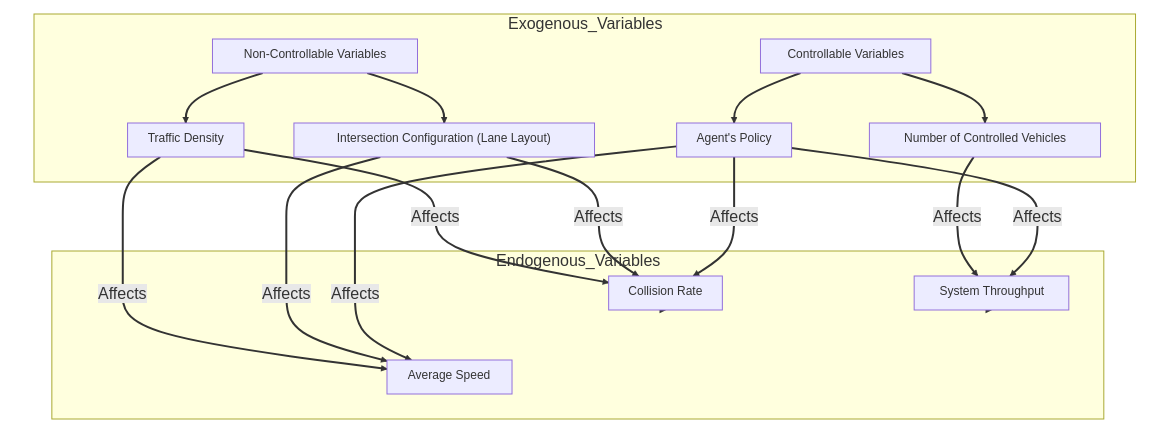
\includegraphics[height=0.25\textheight]{images/variables.png} 
    \caption{System Variables}
\end{figure}



\textbf{State of the System}:

The state of the system at any given time would include a collection of variables such as the number of vehicles in the system, traffic density, the intersection configuration, and the real-time position and speed of each vehicle. 

The state contains all the necessary information to describe the system's current dynamics and predict future behaviors.
      
These elements collectively define how the simulation operates, how decisions are made, and how the performance of the system is evaluated.



\section{Agent Training Algorithms and Policies to be Tested}

The simulation project will consist of three groups, each containing four agents trained using Deep Reinforcement Learning (DRL) techniques based on the \textbf{DQN} and \textbf{PPO} algorithms, employing different policies (\textit{MlpPolicy}, \textit{CnnPolicy}, and \textit{Social Attention Mechanisms}).

The behavior of these agents and their respective policies will be evaluated against a \textbf{Baseline Scenario}, where agents operate without any guiding policy and perform random actions.

\subsection{Training Algorithms}

\subsubsection{1.Deep Reinforcement Learning using DQN}

The Deep Q-Network (DQN) algorithm is a reinforcement learning approach designed to enable agents to learn optimal policies by estimating the value of action-state pairs~\cite{mnih2015dqn}. This is achieved by leveraging neural networks to approximate Q-values, which guide the agent's actions to maximize long-term rewards.

To understand DQN, we first define the concept of a Markov Decision Process (MDP). An MDP is characterized by states \(s\), actions \(a\), rewards \(r\), and transitions \(P(s' \mid s, a)\). The goal in an MDP is to maximize the cumulative reward (also known as the return) over time.

The Q-function represents the expected return of taking a specific action \(a\) in a given state \(s\), followed by an optimal sequence of actions:

\[
Q(s, a) = \mathbb{E} \left[ r_t + \gamma \max_{a'} Q(s_{t+1}, a') \mid s_t = s, a_t = a \right]
\]

Here:
- \(Q(s, a)\) is the value of taking action \(a\) in state \(s\),
- \(r_t\) is the immediate reward received,
- \(\gamma\) is the discount factor, where \(0 \leq \gamma \leq 1\), balancing the importance of immediate and future rewards.

The Q-function is recursively defined using the Bellman equation:

\[
Q(s, a) = r + \gamma \max_{a'} Q(s', a')
\]

In practice, DQN approximates the Q-function using a deep neural network parameterized by \(\theta\):

\[
Q(s, a; \theta) \approx Q^*(s, a)
\]

where \(Q^*(s, a)\) represents the optimal Q-function. 

The neural network learns the parameters \(\theta\) by minimizing the difference between predicted and target Q-values.


\subsubsection{2.Deep Reinforcement Learning using PPO}

Proximal Policy Optimization (PPO) is a reinforcement learning algorithm that aims to improve the policy of an agent by balancing exploration and exploitation\cite{schulman2017ppo}. 
PPO achieves this by using a clipped objective function to prevent large policy updates, ensuring stable learning.

\textbf{Policy Function}

The policy function \(\pi_\theta(a \mid s)\) defines the probability of taking action \(a\) in state \(s\) according to the policy parameters \(\theta\):

\[
\pi_\theta(a \mid s) = \mathbb{P}(a \mid s; \theta)
\]

Here, \(\theta\) parameterizes the policy network. In PPO, the goal is to maximize cumulative rewards while ensuring stability by limiting updates using a clipped objective function.

\textbf{PPO Objective Function}

The objective function used in PPO is a clipped surrogate objective, which aims to optimize the policy by maximizing the expected advantage, but with a constraint on the update size:

\[
L(\theta) = \mathbb{E}_t \left[ \min \left( r_t(\theta) A_t, \text{clip}(r_t(\theta), 1-\epsilon, 1+\epsilon) A_t \right) \right]
\]

Where:
- \(r_t(\theta)\) is the probability ratio between the new and old policy, defined as:

\[
r_t(\theta) = \frac{\pi_\theta(a_t \mid s_t)}{\pi_{\theta_{\text{old}}}(a_t \mid s_t)}
\]

- \(\epsilon\) is the clipping parameter, controlling how much the policy is allowed to change.
- \(A_t\) is the advantage estimate at time step \(t\), which measures how much better an action is compared to the average action.


\subsection{Agent Policies}

We will compare agents' behavior based on four distinct policies:

\begin{enumerate}
    \item\textbf{Baseline {No Policy}}

    \item\textbf{MlpPolicy (Multi-Layer Perceptron Policy)}
    
    The \textit{MlpPolicy} utilizes a multi-layer perceptron neural network to process environmental observations and make decisions. This policy focuses on key input features, such as speed, distance to other vehicles, and intersection layout, allowing agents to act based on their immediate surroundings.

    \textbf{Scenario}: Agents following the \textit{MlpPolicy} will navigate the intersection by leveraging their observed features, applying learned behaviors to respond effectively to dynamic traffic conditions.

    \textbf{Objective}: Assess the performance of \textit{MlpPolicy} agents in terms of efficiency (e.g., throughput, wait times) and safety (e.g., collision rates) compared to agents using other policies. Analyze the influence of input features on their decision-making processes.

    \item\textbf{CnnPolicy (Convolutional Neural Network Policy)}
    
    The \textit{CnnPolicy} employs convolutional neural networks to process visual and spatial data, making it particularly effective in scenarios where visual inputs (like grid representations of the intersection) are crucial for decision-making.

    \textbf{Scenario}: Agents using the \textit{CnnPolicy} will interpret complex visual representations of their environment, allowing them to make informed decisions regarding lane changes, merging, and crossing orders.

    \textbf{Objective}: Evaluate the performance of \textit{CnnPolicy} agents in diverse traffic patterns, focusing on their ability to recognize spatial configurations and respond appropriately to traffic dynamics.

    \item\textbf{Social Attention Mechanisms Policy}
    
    This policy integrates social attention mechanisms, allowing agents to observe and interpret the behaviors and intentions of nearby vehicles. 

Social Attention Mechanisms in Deep Reinforcement Learning (DRL) are inspired by how humans or animals interact within a social environment.
In the context of multi-agent systems, the idea is to integrate social information, allowing agents to pay attention to the behavior and 
intentions of other agents.\cite{sutton2018reinforcement}
This concept helps improve cooperation, communication, and coordination between agents in environments where agents need to share space and interact with each other, such as autonomous vehicles in a traffic intersection.


\paragraph{Attention Mechanisms} 
In deep learning, attention mechanisms allow models to focus on important parts of the input data when making decisions, 
rather than processing everything equally\cite{vaswani2017attention}. 
This is especially useful in scenarios involving sequences or spatial relations, where certain elements might be more significant than others.

\paragraph{Social Attention Mechanisms} 
Social attention mechanisms focus on enabling agents to learn which other agents (or parts of the environment) are most relevant to their actions. 
In the case of DRL with DQN (Deep Q-Network), these mechanisms could take into account the actions and states of surrounding agents when determining a given agent's own actions. 
Essentially, the agent learns a social context that goes beyond its immediate environment\cite{jiang2018learning}.


\paragraph{State Representation with Social Attention} 
In a multi-agent setting, an agent’s state at time $t$, $s_t$, may include not only its own environment but also the states of surrounding agents. Let the state of agent $i$ be represented as $s_i(t)$, and the full state of the environment, including information from other agents, can be written as:
\[
s_t = \{s_i(t), s_{-i}(t)\}
\]
where $s_{-i}(t)$ represents the states of all other agents in the environment at time $t$\cite{mnih2015dqn}.

\paragraph{Social Attention Weights} 
A key idea in social attention is to compute attention weights that determine how much focus an agent should place on each neighboring agent. Let $\alpha_i$ be the attention weight for agent $i$. These weights are learned through a neural network that estimates the importance of each neighboring agent's state in the context of the decision-making process. A common approach is to use a weighted sum, where each agent’s state is weighted according to its relevance:
\[
\tilde{s}_t = \sum_{i \in N} \alpha_i s_i(t)
\]
where $N$ is the set of neighboring agents, and $\alpha_i$ is the attention weight for agent $i$. This process enables each agent to selectively attend to those agents whose states or actions influence its own behavior.

\paragraph{Modifying the Q-Function with Attention} 
The standard DQN Q-function estimates the expected return for each action given a state $s_t$. With the incorporation of social attention, we modify the Q-function to account for the social context:
\[
Q(s_t, a_t) = \mathbb{E}\left[r_t + \gamma \max_{a_{t+1}} Q(s_{t+1}, a_{t+1}; \theta) \mid s_t, a_t\right]
\]
where $s_t$ now includes the social context $\tilde{s}_t$, representing the attention-weighted sum of the agent’s own state and the states of the other agents. The DQN network then estimates the Q-values with this enriched state.

\paragraph{Multi-Head Attention Implementation}
The attention mechanism utilizes multiple heads to compute context-sensitive embeddings, allowing the model to attend to different aspects of the input simultaneously. Each head processes the embeddings independently and outputs its own context-aware representation. The outputs from all heads are concatenated and projected to form the final embedding. The attention computation for each head is given by\cite{DBLP}:
\[
\text{output} = \sigma \left( \frac{Q K^T}{\sqrt{d_k}} \right) V
\]
where:
\[
Q = L_q(e_0), \; K = L_k(e_i), \; V = L_v(e_i)
\]

In these equations:
- $e_i$ denotes the encoded state of vehicle $i$, while $e_0$ corresponds to the ego-vehicle
- $K$ (keys) represents descriptive features of surrounding vehicles
- $V$ (values) contains the embedded features used to compute the final output
- $L_q$, $L_k$, $L_v$ are shared linear projections applied to all vehicles' embeddings
- $\sigma$ is the softmax activation, normalizing attention scores across all vehicles
- $d_k$ represents the dimension of the key embeddings

The ego-vehicle query $Q$ interacts with keys $K$ to compute attention weights, prioritizing vehicles that are most relevant to the ego-vehicle's current context. This results in a weighted combination of values $V$. The outputs from each head are aggregated and passed through a linear layer to produce the final representation.


    This approach helps agents develop cooperative strategies and optimize their interactions with other vehicles. 
    The attention architecture was introduced to enable neural networks to discover inter-dependencies within a variable number of inputs\cite{vaswani2017attention}.



    
    \textbf{Scenario}: Agents utilizing this policy will actively monitor the behavior of surrounding vehicles, adapting their actions based on predicted movements and intentions of others.

    \textbf{Objective}: Investigate the effectiveness of social attention in enhancing cooperation among agents, potentially leading to improved traffic flow and reduced collision rates. 
    Compare the performance of agents using Social Attention Mechanisms against those following other policies to assess their overall effectiveness in a multi-agent environment.
\end{enumerate}


\section{Testing Framework for Operation Policies (Scenarios)}

\begin{enumerate}
    \item \textbf{Experimental Scenarios:} Each policy will be tested under various conditions, such as:
    \begin{itemize}
        \item \textbf{High Traffic Density:} Increased number of vehicles entering the intersection simultaneously.
        \item \textbf{Low Traffic Density:} Sparse vehicle presence to evaluate agent behavior in less congested environments.
    \end{itemize}
    \item \textbf{Group Configuration:} Each group, consisting of four agents using the same policy, will be tested in each scenario. This allows for direct comparisons between the different policies under identical traffic conditions.
    \item \textbf{Performance Metrics:}
    \begin{enumerate}
        \item \textbf{Efficiency:} Metrics such as throughput (vehicles per time unit), and average speed of agents.
        \item \textbf{Safety:} Collision rates, near-misses, and compliance with traffic rules.
        \item \textbf{Adaptability:} How well agents generalize their learned behaviors to new traffic scenarios (e.g., changes in traffic density, lane configurations).
    \end{enumerate}
\end{enumerate}


\section{Global Key Performance Indicators (KPI)}

The following Key Performance Indicators (KPIs) and decision criteria will be used to effectively assess the performance and effectiveness of the operational policies:

\begin{enumerate}
    \item \textbf{Traffic Flow Efficiency}
    \begin{itemize}
        \item \textbf{Metric:} Average vehicle throughput (Arrived vehicles per test episode)
        \item This metric measures how well the intersection handles traffic. A higher throughput indicates that the system is efficiently managing vehicle movement.
    \end{itemize}
    
    \item \textbf{Safety Metrics}
    \begin{itemize}
        \item \textbf{Metric:} Collision rate (Average number of collisions per test episode)
        \item This is a crucial indicator of how safe the intersection is for autonomous vehicles. Reducing collisions is a primary goal for any traffic management system.
    \end{itemize}
    
    \item \textbf{Adaptability to Varying Traffic Conditions}
    \begin{itemize}
        \item \textbf{Metric:} Performance variance (e.g., comparing metrics like wait times and throughput under different traffic densities)
        \item This evaluates how well agents can adjust their behavior to different traffic conditions, ensuring the system's flexibility in dynamic environments.
    \end{itemize}
\end{enumerate}



\chapter{Methodology}
\section{Approach}

This project consists of three key stages, each with specific goals that contribute to the overall aim of developing a robust and adaptable Multi-Agent System (MAS) for managing autonomous vehicles at road intersections. 
The stages are as follows:

\begin{figure}[H]
    \centering
    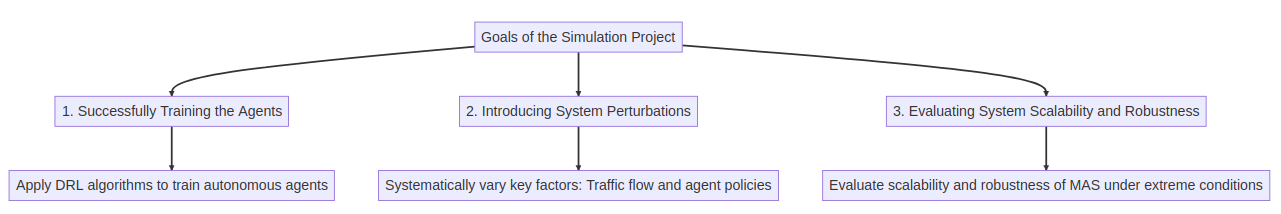
\includegraphics[height=0.12\textheight]{images/goals.png} 
    \caption{Project Methodology}
\end{figure}

\begin{enumerate}
    \item \textbf{Successfully train the agents}

       In this phase, we will apply selected Deep Reinforcement Learning (DRL) algorithms to train autonomous agents in navigating a road intersection.
       
       The agents will learn to make decisions related to intersection crossing order and speed control, with the goal of optimizing traffic flow and avoiding collisions.
           
    \item \textbf{Introducing System Perturbations}
    
   At this stage, the goal is to understand how our different agent policies (policy refers to the strategy/mapping in each agent from state to action) perform when presented with different environment configurations. When it comes to the environment, we tested with two different traffic flow configurations, 
   which we defined as \textbf{sparse} (4 ego vehicles, few other vehicles) or \textbf{dense} (4 ego vehicles, many other vehicles). 
   The goal is to understand if the difference in configuration will alter the algorithm's performance and/or if any of the algorithms are more robust to the changes than others.
       

       
    \item \textbf{Evaluate system scalability and robustness}

    Having trained our learning models, we can load them into the environment and use the approximated policy to make decisions. 
    We run a select number of simulations use this policy and gather metrics from the environment, 
    which are used to compare and evaluate each of the learning algorithms.
\end{enumerate}


\section{Successfully train the agents}


\subsection{Reinforcement Learning Training Process}

\begin{figure}[H]
    \centering
    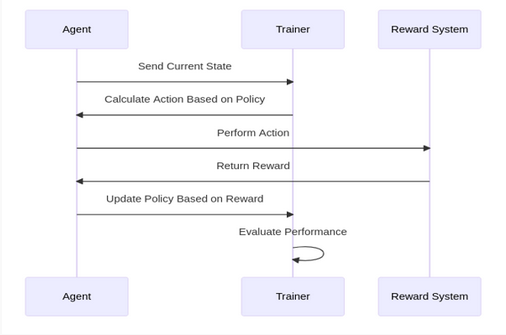
\includegraphics[height=0.25\textheight]{images/train.png} 
    \caption{RL Training Process Sequence}
\end{figure}

The Training Process Sequence can be described as follows:

\subsubsection{1.Initialization}
\begin{itemize}
    \item \textbf{Environment Setup}: An environment is defined (e.g., a traffic intersection using Highway-Env), which provides the observation and action spaces. The environment simulates the interactions of agents and their surroundings.
    \item \textbf{Observation Space}: This defines what the agent perceives at each timestep. For example:
    \begin{itemize}
        \item In the traffic environment, the observation may include a grayscale image of the environment (shape: \((128, 64)\)), stacked over 4 frames to provide temporal context.
        \item The observations are preprocessed to include essential information, such as vehicle positions, velocities, and surrounding traffic.
    \end{itemize}
    \item \textbf{Action Space}: The possible actions an agent can take at each timestep, such as accelerating, braking, or changing lanes in the traffic context.
    \item \textbf{Reward Function}: Rewards guide the agent's learning by providing feedback. The reward is carefully designed to encourage desired behaviors, such as:
    \begin{itemize}
        \item Minimizing travel time.
        \item Avoiding collisions.
        \item Yielding or cooperating with other agents.
    \end{itemize}
\end{itemize}

\subsubsection{2.Agent Initialization}
\begin{itemize}
    \item An RL agent, such as one trained using the Deep Q-Network (DQN) or Proximal Policy Optimization (PPO) algorithm, is instantiated.
    \item The agent interacts with the environment through a defined policy. For example:
    \begin{itemize}
        \item \textbf{DQN}: Uses a neural network to approximate the Q-function, mapping states and actions to expected future rewards.
        \item \textbf{PPO}: Optimizes the policy directly, ensuring stable updates with a clipped objective function.
    \end{itemize}
\end{itemize}

\subsubsection{3.Interaction with the Environment}
At each timestep:
\begin{itemize}
    \item \textbf{Observation}: The agent observes the current state of the environment.
    \item \textbf{Action Selection}: Based on the observation, the agent selects an action using its policy (e.g., an \(\epsilon\)-greedy policy in DQN).
    \item \textbf{Environment Response}: The environment executes the action and provides:
    \begin{itemize}
        \item The next state.
        \item A reward signal.
        \item A flag indicating whether the episode has ended.
    \end{itemize}
\end{itemize}

\subsubsection{4.Experience Storage}
\begin{itemize}
    \item The agent stores experiences as tuples \((s, a, r, s')\) in a replay buffer (for DQN) or uses the trajectory for on-policy updates (PPO).
\end{itemize}

\subsubsection{5.Policy Optimization}
\begin{itemize}
    \item \textbf{DQN}:
    \begin{itemize}
        \item A mini-batch of experiences is sampled from the replay buffer.
        \item The Q-function is updated using the Bellman equation:
        \begin{equation}
        Q(s, a) \leftarrow r + \gamma \max_{a'} Q(s', a')
        \end{equation}
        \item The agent minimizes the temporal difference error between predicted and target Q-values.
    \end{itemize}
    \item \textbf{PPO}:
    \begin{itemize}
        \item The agent computes the advantage function to estimate the relative value of actions.
        \item Policy and value networks are optimized using the PPO loss:
        \begin{equation}
        L(\theta) = \mathbb{E}_t\left[ \min \left( r_t(\theta) A_t, \text{clip}(r_t(\theta), 1-\epsilon, 1+\epsilon) A_t \right) \right]
        \end{equation}
        \item The clipping ensures stable updates.
    \end{itemize}
\end{itemize}

\subsubsection{6.Evaluation and Improvement}
\begin{itemize}
    \item At regular intervals, the agent's policy is evaluated in the environment to assess its performance.
    \item Metrics such as mean reward and train loss are used to gauge improvement.
    \item The best-performing model is saved during training for deployment.
\end{itemize}

\subsubsection{7.End of Training}
\begin{itemize}
    \item After reaching the desired number of training timesteps, the final policy is saved.
    \item Post-training evaluations are conducted to ensure the agent generalizes well to unseen scenarios.
\end{itemize}


\newpage

\subsection{Practical Training Implementation - Configuration}

The training of each agent using the "standard" DQN and PPO algorithms was conducted with \textbf{Stable-Baselines3}\cite{stable-baselines3} within 
a custom multi-agent environment created using the \textbf{Highway-Env} library.

\subsubsection{DQN and PPO with CnnPolicy }

\subsubsection{1.Initialization}

Environment Setup, Observation Space (Python coded): 

\begin{lstlisting}[style=python]
    env = make_vec_env(
        "intersection-v0", 
        n_envs=n_cpu, 
        vec_env_cls=SubprocVecEnv, 
        env_kwargs={
            'config':{
                'initial_vehicle_count': 10,
                'controlled_vehicles': 4,
                'destination': 'o1',
                "observation": {
                    "type": "GrayscaleObservation",
                    "observation_shape": (128, 64),
                    "stack_size": 4,
                    "weights": [0.2989, 0.5870, 0.1140],  # weights for RGB conversion
                    "scaling": 1.75,
                },
            },
        }
    )
\end{lstlisting}

Each environment comes with a default observation, which can be changed or customised using environment configurations. 
In the intersection environment, in order to use the images needed for CNN, the observation type must be defined as \textit{GrayscaleObservation}.

The \textit{GrayscaleObservation} is a \( W \times H \) grayscale image of the scene, where \( W \) and \( H \) are set with the \textit{observation\_shape} parameter. 
The RGB to grayscale conversion is a weighted sum configured by the \textit{weights} parameter. 
Several images can be stacked with the \textit{stack\_size} parameter.



The \textbf{Action Space} is configured as:

\begin{lstlisting}[style=python]
'action': {'lateral': False,
            'longitudinal': True,
            'target_speeds': [0, 4.5, 9],
            'type': 'DiscreteMetaAction'},
\end{lstlisting}

In the default configuration of the intersection environment, only the speed is controlled by the agent, 
while the lateral control of the vehicle is automatically performed by a steering controller to track a desired lane.

So, in this environment the Action Space is defined as:

\begin{lstlisting}[style=python]
ACTIONS= {
        0: 'IDLE',
        1: 'SLOWER',
        2: 'FASTER'
    }
\end{lstlisting}

The \textbf{Reward Function} is focused focus on two features: a vehicle should:

    progress quickly on the road;

    avoid collisions.

Thus, the reward function is composed of a velocity term and a collision term:
\[
R(s,a) = a \left( \frac{v - v_{\min}}{v_{\max} - v_{\min}} \right) - b \text{ collision}
\]

where \( v \), \( v_{\min} \), and \( v_{\max} \) are the current, minimum, and maximum speed of the ego-vehicle respectively, and \( a \), \( b \) are two coefficients.

In practical terms the following rewards are used in this environment:
\begin{lstlisting}[style=python]
    'arrived_reward': 1,
    'collision_reward': -5,
    'high_speed_reward': 1
\end{lstlisting}

Being the final episode reward calculated as an average of the reward of all controlled agents.

\subsubsection{2.1 - Agent Initialization for DQN algorithm using CnnPolicy}

The following parameters have been used in the training processes with CnnPolicy :

\begin{lstlisting}[style=python]
    model = DQN(
        "CnnPolicy",
        env,
        learning_rate=5e-4,
        buffer_size=15000,
        learning_starts=200,
        batch_size=32,
        gamma=0.8,
        train_freq=1,
        gradient_steps=1,
        target_update_interval=50,
        exploration_fraction=0.7,
        verbose=2,
        tensorboard_log=model_dir,
    )
\end{lstlisting}

\subsubsection{2.2 - Agent Initialization for PPO algorithm using CnnPolicy}

\begin{lstlisting}[style=python]
    batch_size = 64
    model = PPO(
        "CnnPolicy",
        env,
        n_steps=batch_size * 12 // n_cpu,
        batch_size=batch_size,
        n_epochs=10,
        learning_rate=3e-4,
        gamma=0.9,
        verbose=2,
        tensorboard_log=model_dir,
    )
\end{lstlisting}

\subsubsection{DQN and PPO with MlpPolicy }

\subsubsection{1.Initialization}

Environment Setup, Observation Space (Python coded): 

\begin{lstlisting}[style=python]
    env = make_vec_env(
        "intersection-v0", 
        n_envs=n_cpu, 
        vec_env_cls=SubprocVecEnv, 
        env_kwargs={
            'config':{
                'vehicles_count': 10,
                'controlled_vehicles': 4,
                'destination': 'o1',
            },
        }
    )

\end{lstlisting}

The MlpPolicy needs a different type of observations: \textit{Kinematics}.

The \textit{KinematicObservation} is a  a \( V \times F \) array  and that describes a list of \( V \) nearby vehicles by a set of features of size  \( F \)
listed in the "features" configuration field. In this particular case we are using:

\begin{lstlisting}[style=python]
'observation': {'absolute': True,
'features': ['presence',
             'x',
             'y',
             'vx',
             'vy',
             'cos_h',
             'sin_h'],
'features_range': {'vx': [-20, 20],
                   'vy': [-20, 20],
                   'x': [-100, 100],
                   'y': [-100, 100]},
'type': 'Kinematics',
}
\end{lstlisting}

where: 

\textit{presence}:Disambiguate agents at 0 offset from non-existent agents.

\textit{x} and \textit{y}: World offset of ego vehicle or offset to ego vehicle on the x and y axis.

\textit{vx} and \textit{vy}: Velocity on the x and y axis of vehicle.

\textit{cos\_h} and \textit{sin\_h}: Trigonometric heading of vehicle.


Which produces an observation array similar to the one represented in the table bellow:

\begin{table}[h!]
    \centering
    \begin{tabular}{|c|c|c|c|c|c|c|c|}
    \hline
    \textbf{Vehicle} & \textbf{presence} & \textbf{x} & \textbf{y} & \textbf{vx} & \textbf{vy} & \textbf{cos\_h} & \textbf{sin\_h} \\ \hline
    ego-vehicle & 1 & 5.0  & 4.0  & 15.0  & 0   & 1  & 0 \\ \hline
    vehicle 1  & 1 & -10.0 & 4.0  & 12.0  & 0   & 1  & 0 \\ \hline
    vehicle 2  & 1 & 13.0  & 8.0  & 13.5  & 0   & 1  & 0 \\ \hline
    ...         & ...   & ...  & ...   & ... & ... & ...& ... \\ \hline
    vehicle V  & 1 & 22.2  & 10.5 & 18.0  & 0.5 & 1  & 0 \\ \hline
    \end{tabular}
    \caption{Example of \textit{Kinematic} observation }
    \label{tab:vehicles}
\end{table}

 The Action Space and Reward Function are similar to those used in the \textit{CnnPolicy} 
    

 \subsubsection{2.1 - Agent Initialization for DQN algorithm using MlpPolicy}

 \begin{lstlisting}[style=python]
    model = DQN(
        "MlpPolicy",
        env,
        learning_rate=3e-4,
        buffer_size=15000,
        learning_starts=200,
        batch_size=32,
        gamma=0.8,
        train_freq=1,
        gradient_steps=1,
        target_update_interval=50,
        exploration_fraction=0.5,
        verbose=2,
        tensorboard_log=model_dir
    )
\end{lstlisting}

\subsubsection{2.2 - Agent Initialization for PPO algorithm using MlpPolicy}

\begin{lstlisting}[style=python]
    batch_size = 64
    model = PPO(
        "MlpPolicy",
        env,
        n_steps=batch_size * 12 // n_cpu,
        batch_size=batch_size,
        n_epochs=10,
        learning_rate=3e-4,
        gamma=0.9,
        verbose=2,
        tensorboard_log=model_dir,
    )
\end{lstlisting}

\subsubsection{Decentralized Social Influence DQN}

As for decentralized training, each agent is represented by its own network (and therefore optimizer, during training). This means that each agent's network is being fitted only to its own actions, rewards and observations, rather than their collective counterparts. This approach can benefit training because when using the collective reward and observation, centralized networks might not be able to capture small changes in actions for each agent. Furthermore, this in turn allows us to use Social Influence, a concept in which each agent's behavior is influenced by others, which we will further explain. 

The key concept is that we are using this neural network as a universal function approximator in order to approximate our theoretical $Q$ function, which we could use to pick the maximum value action for each state. We assume the fact that every $Q$ function obeys the \textit{Bellman Equation}:
\[
Q^\pi(s, a) = r + \gamma Q^\pi(s', \pi(s'))
\]
From this, we get the temporal difference error, $\delta$, which is what we attempt to minimize:
\[
\delta = Q(s, a) - \left(r + \gamma \max_{a'} Q(s', a')\right)
\]

The training pipeline for this approach follows closely \cite{pytorch_rl_tutorial}. Each agent is represented by its own policy network and target network. We select actions according to an epsilon greedy policy, using Replay Memory to store transitions of the type \textit{(State, Action, Next State, Reward}. By obtaining a batch of these transitions for each autonomous agent, we optimize the network by minimizing the \textit{Huber Loss} calculated with respect to the previously mentioned $delta$:

\[
L = \frac{1}{|B|} \sum_{(s, a, s', r) \in B} L(\delta),
\]
where
\[
L(\delta) =
\begin{cases} 
\frac{1}{2}\delta^2 & \text{for } |\delta| \leq 1, \\
|\delta| - \frac{1}{2} & \text{otherwise}.
\end{cases}
\]

where $(s, a, s', r)$ is a single transition.

Having succesfully achieve decentralized training, the next step would be to implemented some kind of social mechanism, given that the agent's have to learn to respond to each other's behavior, in particular in an road intersection scenario. We chose to implement what is known as the \textit{Basic Social Influence} mechanism from \cite{jaques2019social}, that shifts agent's rewards using counterfactuals, so that it becomes $r^k_t = \alpha e^k_t + \beta c^k_t$ where $e^k_t$ is the extrinsic or environmental reward, and $c^k_t$ is the causal influence reward.  Essentially, agent \textit{k} asks the question: “How would \textit{j’s} action change if I had acted differently in this situation?”. This causal influence rewards is obtained by calculating the divergence between the marginal policy of j (if \textit{j} did not consider \textit{k}) and the conditional policy of \textit{j} (when \textit{j} does consider \textit{k}).

\begin{figure}[h]
    \centering
    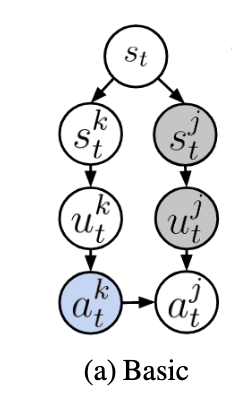
\includegraphics[scale=0.5]{social_influence.png}
    \caption{Chain of social influence}
    \label{fig:social influence}
\end{figure}

\subsection{Practical Training Implementation - Execution and Results}

The previously configured models were trained for a minimum of 1 million timesteps or until the average reward reached its maximum value. 
At regular intervals, the agent's policy was evaluated within the environment to assess its performance,
and the model was saved whenever the metrics improved. 
Metrics such as mean reward and training loss were used to measure progress.

The training process was monitored using TensorBoard. 
For each training session, the evolution of the average reward and the train loss were displayed. 
Below are the logs of these processes:


\subsubsection{DQN}

1. DQN with CnnPolicy

\begin{figure}[H]
    \centering
    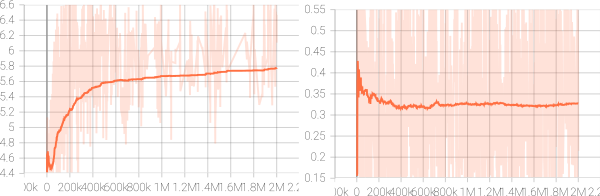
\includegraphics[height=0.20\textheight]{images/dqn_cnn.png} 
    \caption{DQN with CnnPolicy training Log - Average Reward and Train Loss Evolution}
\end{figure}



2. DQN with MlpPolicy

\begin{figure}[H]
    \centering
    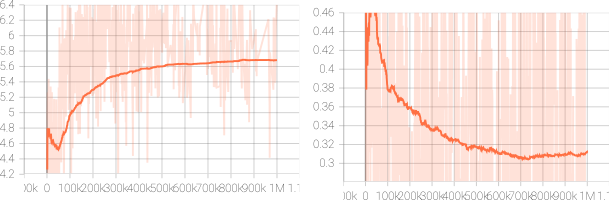
\includegraphics[height=0.20\textheight]{images/dqn_mlp.png} 
    \caption{DQN with MlpPolicy training Log - Average Reward and Train Loss Evolution}
\end{figure}

\subsubsection{PPO}

1. PPO with CnnPolicy

\begin{figure}[H]
    \centering
    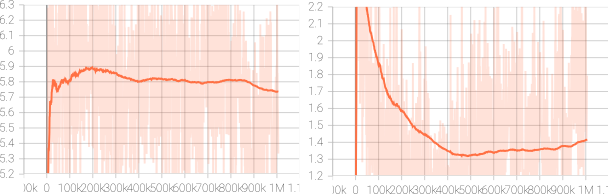
\includegraphics[height=0.20\textheight]{images/ppo_cnn.png} 
    \caption{PPO with CnnPolicy training Log - Average Reward and Train Loss Evolution}
\end{figure}



2. PPO with MlpPolicy

\begin{figure}[H]
    \centering
    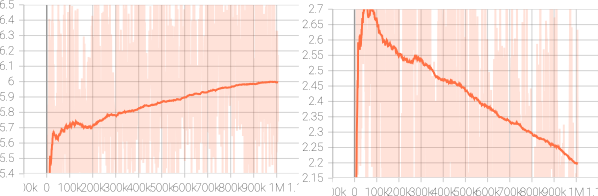
\includegraphics[height=0.20\textheight]{images/ppo_mlp.png} 
    \caption{PPO with MlpPolicy training Log - Average Reward and Train Loss Evolution}
\end{figure}


\section{Introducing System Perturbations}

\subsection{Pipeline for Agent Policy Evaluation}

The primary goal of this study is to understand how different agent policies perform when presented with various and unseen environment configurations. 
To achieve this, we tested the agents with two distinct traffic flow configurations: sparse (featuring 4 ego vehicles and a few other vehicles) 
and dense (featuring 4 ego vehicles and many other vehicles). 

We have developed a pipeline that encompasses the following steps:
\begin{itemize}
    \item Load and test the different trained models.
    \item Simulate different environment configurations.
    \item Record the videos of these simulations.
    \item Calculate and plot the episode metrics.
    \item Calculate and plot the global average metrics and indicators.
\end{itemize}

This pipeline has been implemented as a \textbf{Streamlit application}, enabling the integration of all these features and facilitating a smooth 
workflow between the various components. In the following sections, we will describe the application in detail.

\begin{figure}[H]
    \centering
    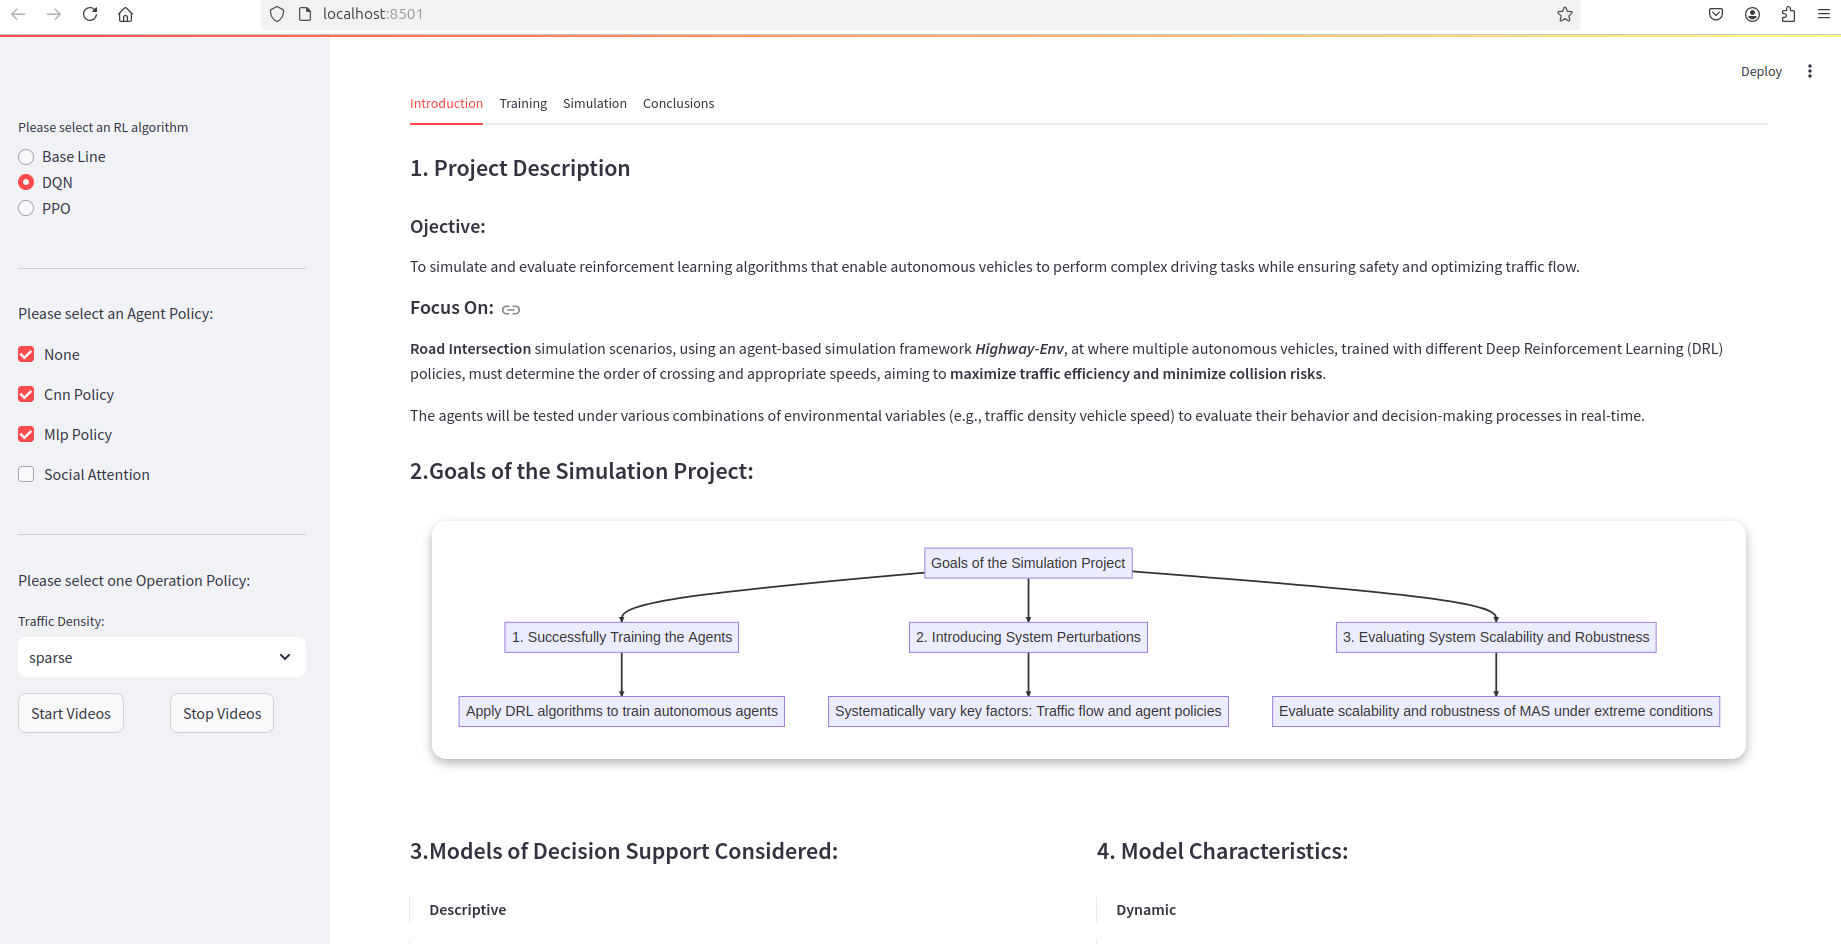
\includegraphics[height=0.35\textheight]{images/app_intro.png} 
    \caption{Streamlit Application - Layout}
\end{figure}


\subsection{Streamlit Application for RL Highway-Env}

The Streamlit application implements the functionality for simulating and analyzing the performance of different agent policies in an intersection environment.
The main goal is to evaluate how the agent's policies perform under various traffic flow configurations, namely sparse and dense traffic. 
The key features and flow of the code are outlined as follows:

\subsubsection{Sidebar Configuration}

The sidebar is a crucial part of the application, allowing users to customize and select the simulation parameters. The sidebar is divided into several sections:

\begin{itemize}
    \item \textbf{RL Algorithm Selection:} 
    Users can select the reinforcement learning (RL) algorithm to be used for the simulation. The available options are:
    \begin{itemize}
        \item \textit{Base Line}
        \item \textit{DQN}
        \item \textit{PPO}
    \end{itemize}

    \item \textbf{Agent Policy Selection:} 
    The user can also select the policy for the agent from a set of options:
    \begin{itemize}
        \item \textit{None} 
        \item \textit{CNN Policy}
        \item \textit{MLP Policy}
        \item \textit{Social Attention}
    \end{itemize}
    
    \item \textbf{Traffic Density Selection:} 
    A dropdown menu lets the user select the traffic density configuration, which can either be:
    \begin{itemize}
        \item \textit{Sparse} (4 ego vehicles and a few other vehicles)
        \item \textit{Dense} (4 ego vehicles with many other vehicles)
    \end{itemize}

    \item \textbf{Video Control:} 
    The sidebar also includes two buttons to control the video playback of the simulation:
    \begin{itemize}
        \item \textit{Start Videos} - Starts the simulation videos
        \item \textit{Stop Videos} - Stops the simulation videos
    \end{itemize}
\end{itemize}

These options allow the user to specify the RL algorithm, agent policy, and traffic density, enabling them to test the performance of different configurations in the environment.

The application is also divided into several tabs, each serving a different purpose for presenting the simulation results and performance metrics. 
These tabs are as follows:

\begin{itemize}
    \item \textbf{Introduction Tab:} 
    This tab provides an overview of the application and its objectives. It introduces the simulation environment, the agent policies being evaluated, and the traffic configurations used for the experiments.
    
    \item \textbf{Training Tab:} 
    Here, users can explore the details of the training process. This section includes some theorethical basis of the train process as well as visualizations,graphs and plots of training results, such as mean rewards and loss functions, to help assess the agent's learning progress.
    
    \begin{figure}[H]
        \centering
        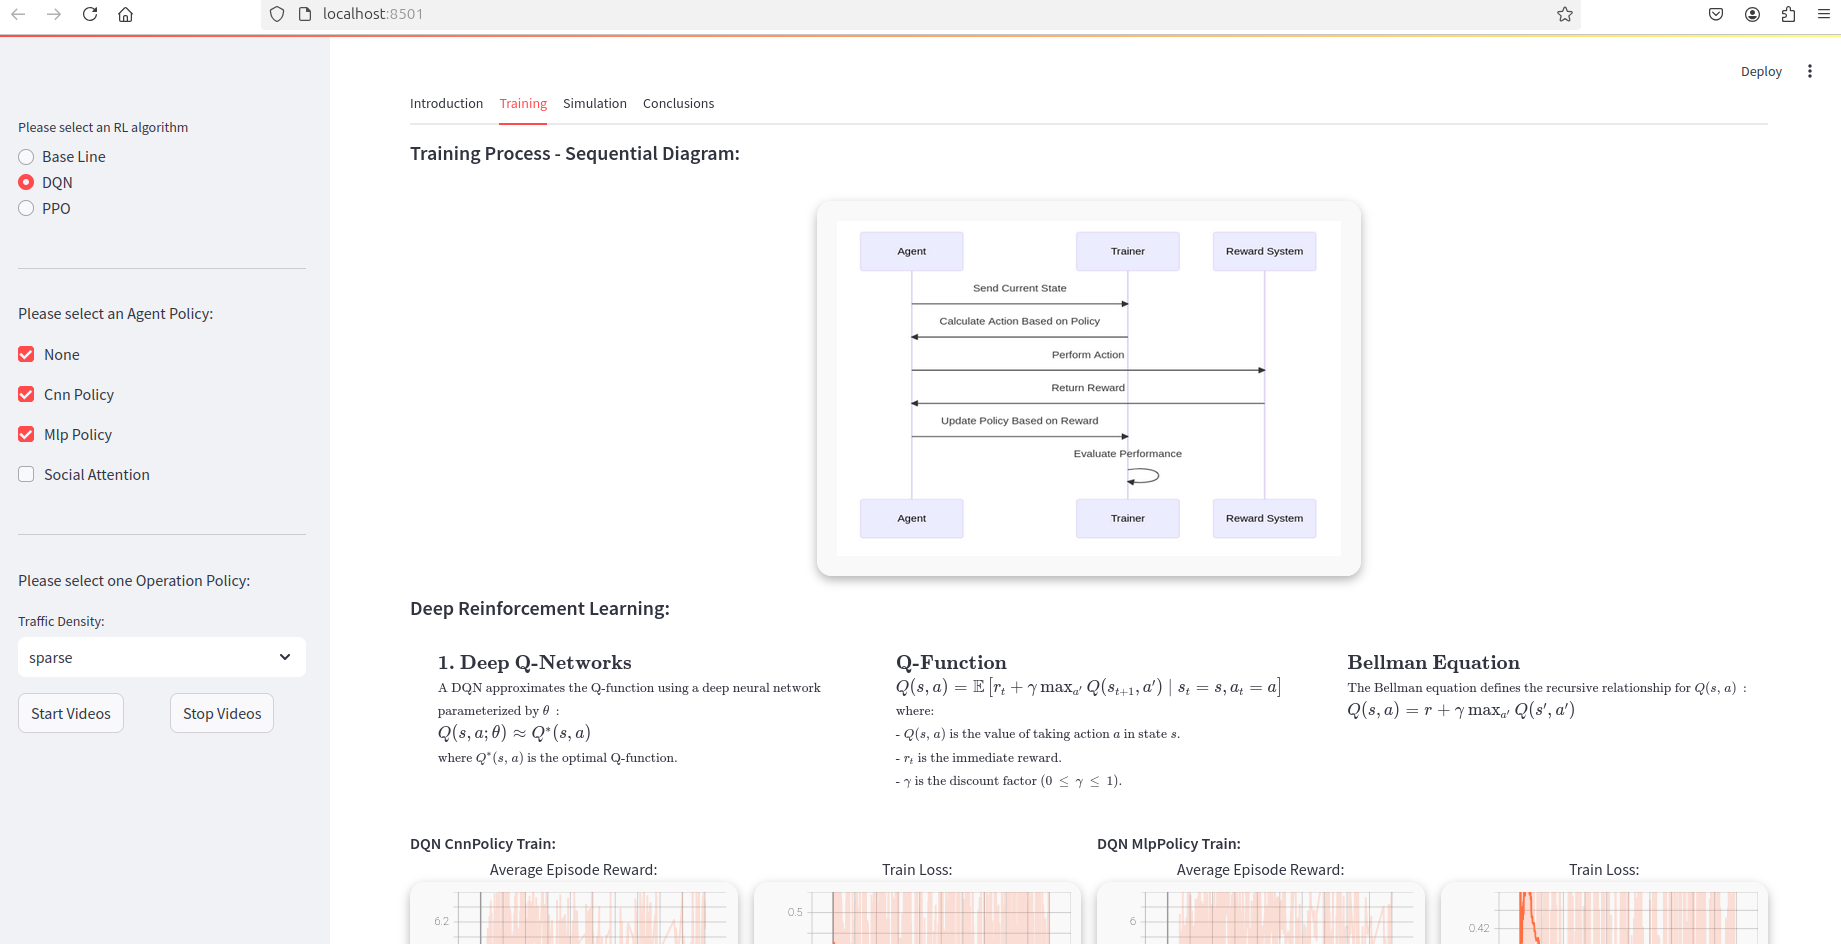
\includegraphics[height=0.35\textheight]{images/app_train.png} 
        \caption{Streamlit Application - Train Tab}
    \end{figure}
    

    \item \textbf{Simulation Tab:} 
    This tab shows the simulation results based on the selected agent policy, algorithm, and traffic configuration. The user can view simulation videos, performance plots, and metrics related to the agent's interaction with the environment.
    
  
    \begin{figure}[H]
        \centering
        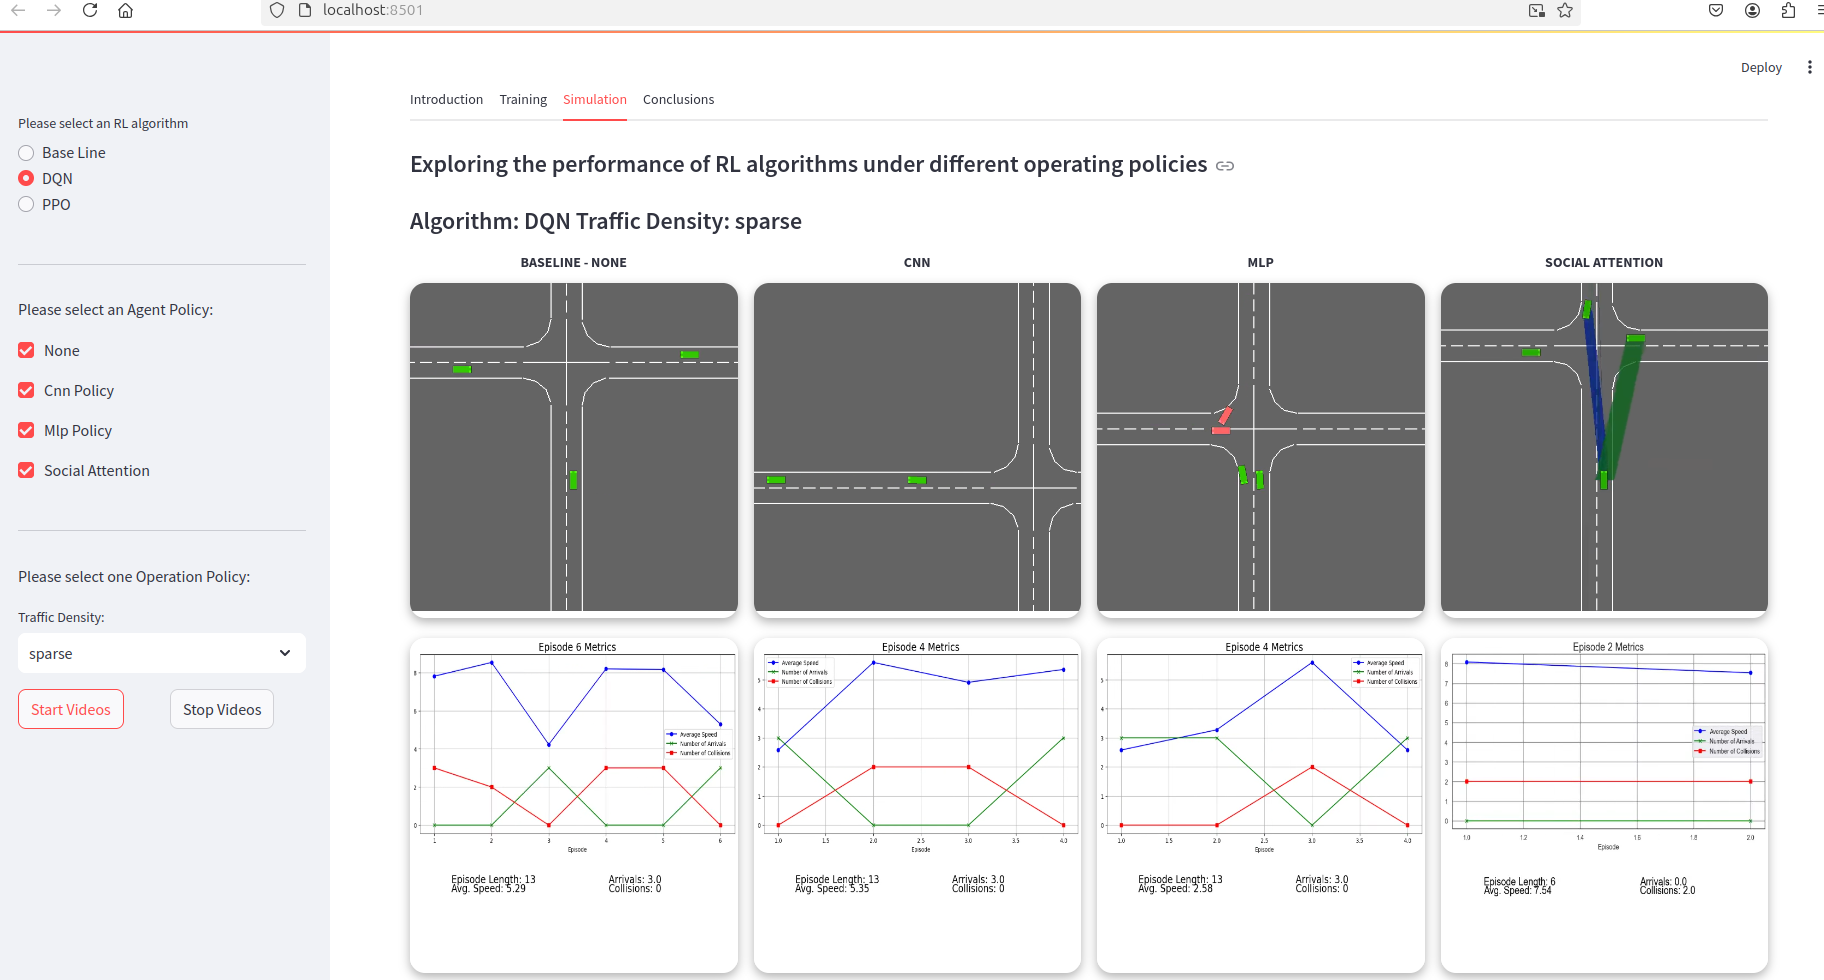
\includegraphics[height=0.35\textheight]{images/app_simulation.png} 
        \caption{Streamlit Application - Simulation Tab}
    \end{figure}
    

    \item \textbf{Conclusions Tab:} 
    This section summarizes the findings of the experiments, discusses the agent's performance under various configurations, and highlights any insights derived from the evaluation.
\end{itemize}

\begin{figure}[H]
    \centering
    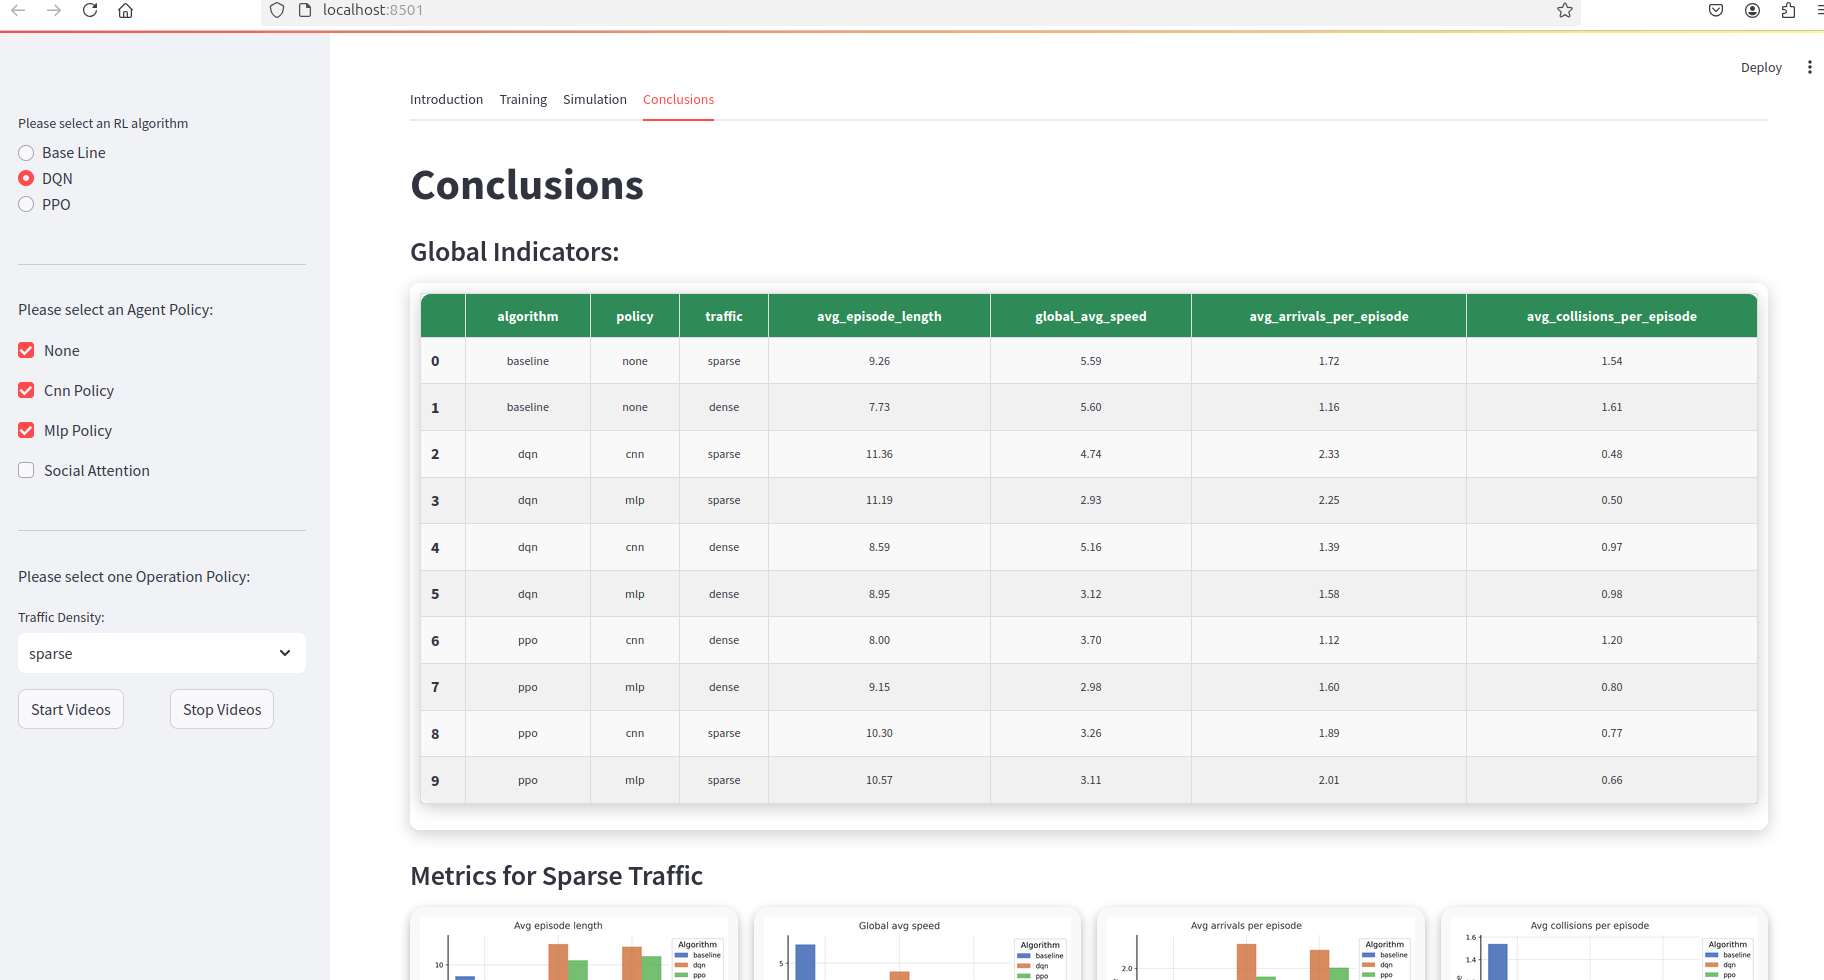
\includegraphics[height=0.35\textheight]{images/app_conclusions.png} 
    \caption{Streamlit Application - Conclusions Tab}
\end{figure}

\newpage

\section{Evaluate system scalability and robustness}

After training the learning models and integrating them into the application, we will utilize the approximated policy to inform decision-making. 

We conduct \textbf{100 simulations} for each algorithm or policy, collecting metrics from the environment based on this policy. 
These metrics allow us to evaluate the performance of the trained model and environment:
\begin{itemize}
    \item \textbf{Local metrics} give insight into the performance of the model within individual episodes, such as how efficiently it minimizes collisions or maximizes arrivals.
    \item \textbf{Global metrics} summarize the overall performance of the model across multiple episodes, useful for comparing different algorithms, policies, or configurations.
\end{itemize}

\subsection{Metrics Description}

\subsubsection*{Local Metrics (per episode)}

\begin{enumerate}
    \item \textbf{Average Speed}:
    \begin{itemize}
        \item \textbf{Description}: The average speed of all agents in the environment during the current episode.
        \item \textbf{Formula}:
        \[
        \text{avg\_speed} =
        \begin{cases}
        \frac{\text{speed\_sum}}{\text{step\_count}}, & \text{if } \text{step\_count} > 0 \\
        0, & \text{otherwise}
        \end{cases}
        \]
    \end{itemize}
    
    \item \textbf{Total Arrived Reward}:
    \begin{itemize}
        \item \textbf{Description}: The cumulative reward for all agents arriving at their destinations during the episode.
        \item \textbf{Formula}:
        \[
        \text{total\_arrived\_reward} = \text{infos}["\text{rewards}"]["\text{arrived\_reward}"]
        \]
        (Directly fetched from the environment's information dictionary).
    \end{itemize}
    
    \item \textbf{Number of Arrivals}:
    \begin{itemize}
        \item \textbf{Description}: The number of vehicles that successfully arrived at their destination in the current episode. 
       
        Each arrival contributes a reward of \(\frac{1}{\text{number\_of\_controlled\_agents}}\), so the number of arrivals is calculated by dividing 
        the total arrived reward by that fraction.

        \item \textbf{Formula}:
        \[
        \text{number\_of\_arrivals} = \frac{\text{total\_arrived\_reward}}{\frac{1}{\text{number\_of\_controlled\_agents}}}
        \]
    \end{itemize}
    
    \item \textbf{Number of Collisions}:
    \begin{itemize}
        \item \textbf{Description}: The number of collisions that occurred during the episode. This is inferred by summing the termination flags of agents (if provided by the environment).
        \item \textbf{Formula}:
        \[
        \text{number\_of\_collisions} = \sum \text{infos}["\text{agents\_terminated}"]
        \]
        (Assumes the termination flag indicates a collision).
    \end{itemize}
\end{enumerate}

\subsubsection*{Global Metrics (across all episodes)}

\begin{enumerate}
    \item \textbf{Global Average Speed}:
    \begin{itemize}
        \item \textbf{Description}: The overall average speed of all agents across all episodes.
        \item \textbf{Formula}:
        \[
        \text{global\_avg\_speed} =
        \begin{cases}
        \frac{\text{total\_speed\_sum}}{\text{total\_step\_count}}, & \text{if } \text{total\_step\_count} > 0 \\
        0, & \text{otherwise}
        \end{cases}
        \]
    \end{itemize}
    
    \item \textbf{Average Arrivals per Episode}:
    \begin{itemize}
        \item \textbf{Description}: The mean number of vehicles that successfully arrived at their destinations per episode.
        \item \textbf{Formula}:
        \[
        \text{avg\_arrivals\_per\_episode} = \frac{\text{total\_arrivals}}{\text{n\_episodes}}
        \]
    \end{itemize}
    
    \item \textbf{Average Collisions per Episode}:
    \begin{itemize}
        \item \textbf{Description}: The mean number of collisions that occurred per episode.
        \item \textbf{Formula}:
        \[
        \text{avg\_collisions\_per\_episode} = \frac{\text{total\_collisions}}{\text{n\_episodes}}
        \]
    \end{itemize}
    
    \item \textbf{Average Episode Length}:
    \begin{itemize}
        \item \textbf{Description}: The mean number of steps (time steps) per episode.
        \item \textbf{Formula}:
        \[
        \text{avg\_episode\_length} = \frac{\text{total\_step\_count}}{\text{n\_episodes}}
        \]
    \end{itemize}
\end{enumerate}

\subsection{Metrics Collection}

The metrics are collected during the environment simulation loop, specifically in the section where the step() function of the environment is called. 

\begin{lstlisting}[style=python]
obs, reward, terminated, truncated, infos = env.step(action)
\end{lstlisting}


The \texttt{step()} function takes the action predicted by the model and advances the environment by one time step. The outputs are:
\begin{itemize}
    \item \texttt{obs}: The new observation (state) after taking the action.
    \item \texttt{reward}: The immediate reward from the environment for the action.
    \item \texttt{terminated}: A boolean indicating if the episode has ended due to termination criteria.
    \item \texttt{truncated}: A boolean indicating if the episode has ended due to a time limit.
    \item \texttt{infos}: A dictionary containing additional information from the environment.
\end{itemize}

After each step, the \texttt{infos} dictionary is used to update various metrics:

\begin{verbatim}
speed_sum += infos['speed']
\end{verbatim}
The speed of the agents at this time step is fetched from the \texttt{infos} dictionary and added to \texttt{speed\_sum}. This accumulates the total speed over the episode.

\begin{verbatim}
step_count += 1
\end{verbatim}
The \texttt{step\_count} variable is incremented with each step to keep track of the number of steps in the episode.

At the end of the episode (when \texttt{terminated} or \texttt{truncated} is \texttt{True}), additional metrics are calculated:

\begin{verbatim}
avg_speed = speed_sum / step_count if step_count > 0 else 0
\end{verbatim}
The total speed accumulated during the episode is divided by the total steps to calculate the average speed.

\begin{verbatim}
total_arrived_reward = infos["rewards"]["arrived_reward"]
number_of_arrivals = total_arrived_reward / (1/number of controlled vehicles)
\end{verbatim}
The total arrived reward is fetched directly from the \texttt{infos} dictionary, and the number of arrivals is derived by dividing this reward by \(0.25\).

\begin{verbatim}
if not truncated:
    final_agents_terminated = infos["agents_terminated"]
    number_of_collisions = sum(final_agents_terminated)
\end{verbatim}
If the episode ended due to termination, the \texttt{agents\_terminated} information from the \texttt{infos} dictionary is used to infer the number of collisions.



The \textbf{global metrics} are computed by aggregating and averaging data collected across all episodes. 

These metrics provide insights into the overall performance of the model.

\begin{itemize}
\item\textbf{Global Average Speed}:The overall average speed of all agents across all episodes.  
\begin{verbatim}
global_avg_speed = total_speed_sum / total_step_count if total_step_count > 0 else 0
\end{verbatim}

\item\textbf{Average Arrivals per Episode} The mean number of vehicles that successfully arrived at their destinations per episode. 
\begin{verbatim}
avg_arrivals_per_episode = total_arrivals / n_episodes
\end{verbatim}


\item\textbf{Average Collisions per Episode} The mean number of collisions that occurred per episode. 
\begin{verbatim}
avg_collisions_per_episode = total_collisions / n_episodes
\end{verbatim}


\item\textbf{Average Episode Length} The mean number of steps (time steps) per episode.
\begin{verbatim}
avg_episode_length = total_step_count / n_episodes
\end{verbatim}
\end{itemize}

These metrics are stored and optionally exported to a CSV file for further analysis. 

They allow for evaluating and comparing the performance of different algorithms, policies, or traffic configurations:
\begin{itemize}
    \item \textbf{Global Average Speed:} Indicates how effectively the model maintains higher speeds across episodes.
    \item \textbf{Average Arrivals per Episode:} Measures how successfully the agents reach their destinations.
    \item \textbf{Average Collisions per Episode:} Tracks the frequency of collisions, highlighting safety concerns.
    \item \textbf{Average Episode Length:} Provides insight into the time efficiency of episodes. Longer episodes means better model performance.
\end{itemize}

During the simulation, the application generates and displays separate plots for the local metrics, enabling a visual comparison of the different algorithms and policies selected by the user. 


\begin{figure}[H]
    \centering
    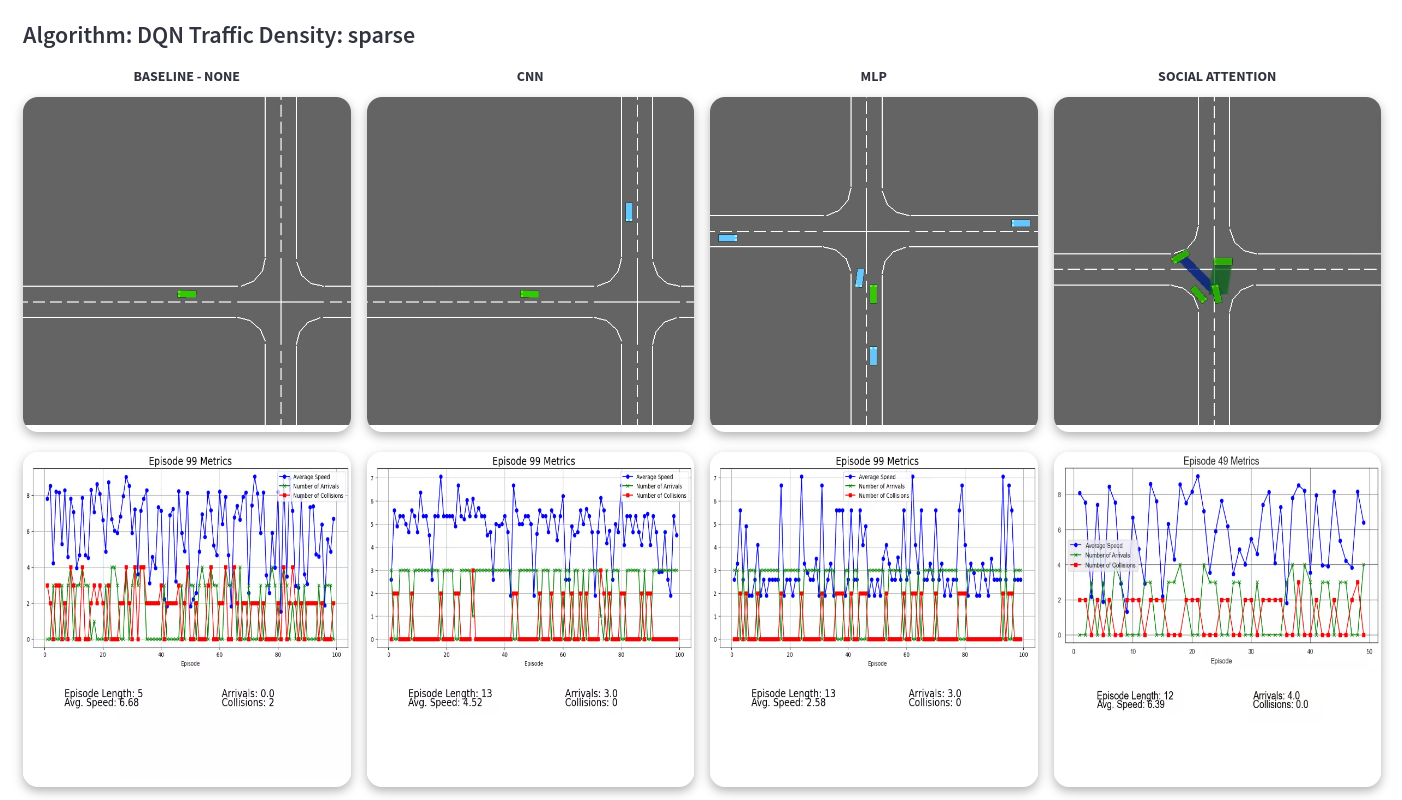
\includegraphics[height=0.4\textheight]{images/app_plots.png} 
    \caption{Simulation - Local Metrics Plot}
\end{figure}

At the conclusion of all episodes, the global metrics for each scenario can also be presented.

\begin{figure}[H]
    \centering
    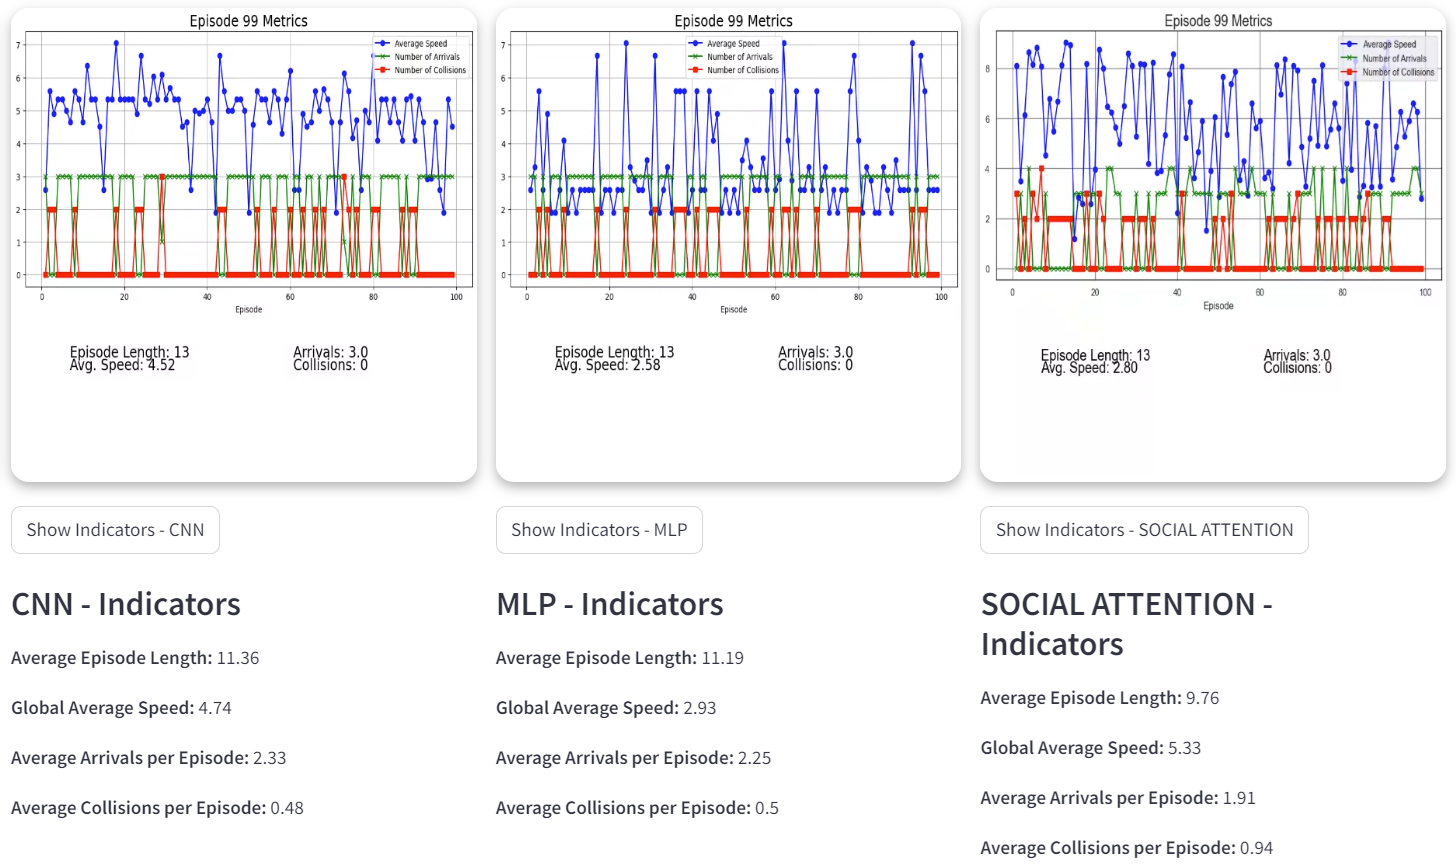
\includegraphics[height=0.4\textheight]{images/app_global_metrics.png} 
    \caption{Simulation - Global Metrics}
\end{figure}





\chapter{Results and Discussion}
\section{Results and Discussion}

After simulating all possible combinations of algorithm, agent policy, and traffic density, the global metrics were collected and are summarized in the table below:

\begin{figure}[H]
    \centering
    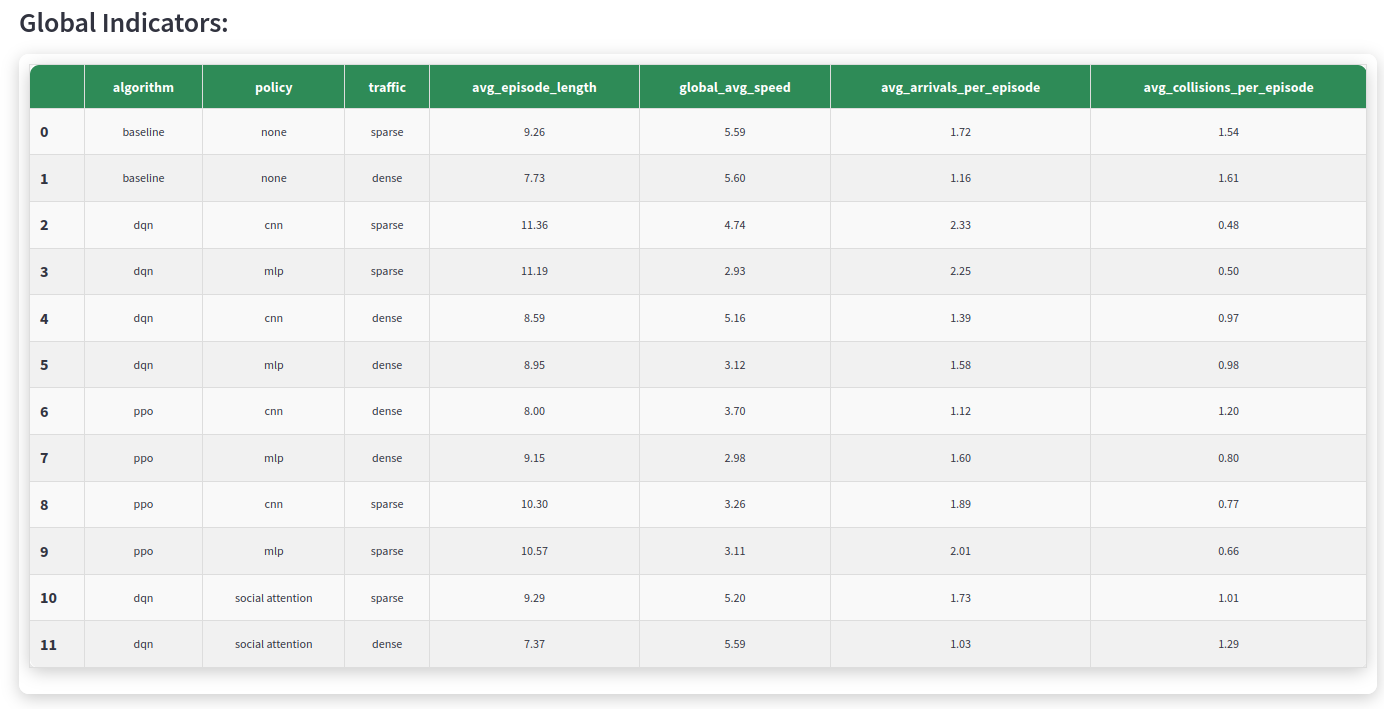
\includegraphics[height=0.42\textheight]{images/app_global_indicators.png} 
    \caption{Summary of Global Metrics for All Algorithm / Policy / Traffic Combinations}
\end{figure}

and plotted:

\begin{figure}[H]
    \centering
    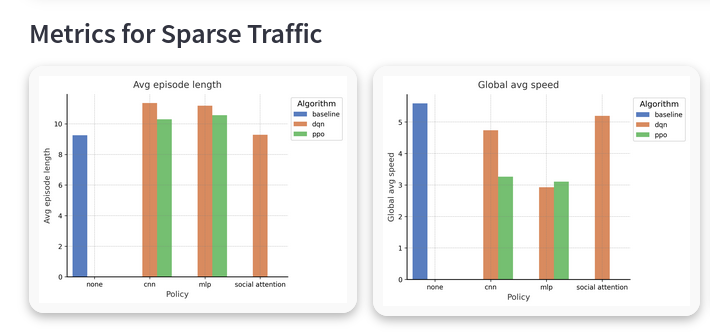
\includegraphics[height=0.22\textheight]{images/app_global_plots_sparse1.png} 
\end{figure}

\begin{figure}[H]
    \centering
    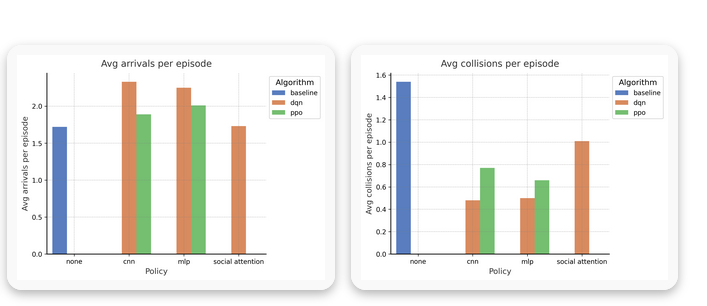
\includegraphics[height=0.19\textheight]{images/app_global_plots_sparse2.png} 
    \caption{Summary of Global Metrics for Sparse Traffic}
\end{figure}

\begin{figure}[H]
    \centering
    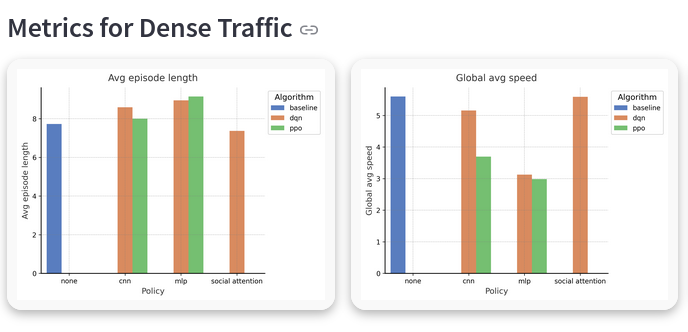
\includegraphics[height=0.215\textheight]{images/app_global_plots_dense1.png} 
\end{figure}

\begin{figure}[H]
    \centering
    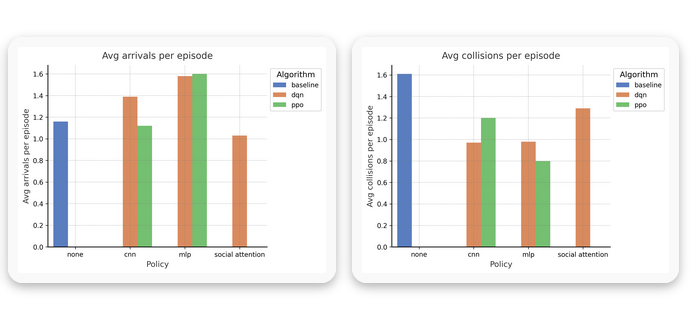
\includegraphics[height=0.2\textheight]{images/app_global_plots_dense2.png} 
    \caption{Summary of Global Metrics for Dense Traffic}
\end{figure}

The results in the table and plots reveal several important trends and insights regarding the performance of the different combinations of algorithm, policy, and traffic density:

\textbf{Average Episode Length}

The average episode length is an important indicator of how well an algorithm handles the traffic conditions without causing early terminations (such as collisions). A longer episode typically suggests that the algorithm is performing well by effectively navigating through the environment, handling traffic without triggering collisions, while shorter episodes may indicate that the agent fails to handle the traffic complexity and encounters more collisions, which results in the early termination of the episode.

In general, the \textbf{average episode length} tends to vary depending on the traffic density, with some algorithms, like PPO, being more resilient in different traffic conditions. These differences in episode length can help evaluate the adaptability of different algorithms to the varying complexities of real-world scenarios, where traffic can range from sparse to dense.
In conclusion, longer episode lengths generally indicate that the algorithms are better at managing traffic randomness and avoiding collisions, leading to smoother, longer episodes. This trend is especially evident in algorithms like DQN, where deeper learning methods tend to produce longer episodes as they allow agents to effectively deal with the traffic complexity. On the other hand, shorter episodes suggest that the algorithm might be struggling with handling the traffic, resulting in earlier episode termination due to collisions.

\textbf{Global Average Speed}

The global reflects the overall efficiency of the agents in the environment. 
It provides an indication of how quickly the agents are able to complete their tasks. 
However, it is essential to consider global average speed in conjunction with other metrics, such as episode length and the number of collisions, 
as a higher speed can sometimes result in more collisions, which would lead to earlier episode terminations.

While higher speeds are generally favorable for achieving higher efficiency, they need to be carefully balanced with the likelihood of collisions and the episode length. 
In this study, the \textbf{baseline} algorithm, which exhibits the highest global speeds, also suffers from shorter episode lengths, suggesting that the increased speed leads to more collisions. 
On the other hand, algorithms like \textbf{dqn} (especially with the \textbf{cnn} and \textbf{mlp} policies) maintain a more balanced speed, leading to longer episodes and fewer collisions. 
This highlights that optimal performance is not solely about speed, but about the balance between speed, collision avoidance, and the ability to handle complex traffic situations.

\textbf{Average Arrivals per Episode and Average Collisions per Episode}

The number of arrivals and collisions are key metrics in assessing the efficiency and safety of the agents' behaviors. 
The total number of arrivals is directly influenced by the number of collisions because the episode ends when a collision occurs, 
which in turn prevents additional arrivals. 
Therefore, these two metrics are inherently linked, with more collisions generally resulting in fewer arrivals.

The number of arrivals is inversely related to the number of collisions, with the highest arrivals typically occurring in configurations that minimize collisions. 
For example, the \textbf{dqn} algorithms, especially with \textbf{cnn} and \textbf{mlp} policies, strike a good balance between speed, collision avoidance, and arrivals, leading to more arrivals due to longer episodes. 
The \textbf{baseline} algorithm, on the other hand, struggles to avoid collisions, leading to fewer arrivals, particularly in dense traffic. 
The \textbf{ppo} algorithm appears less efficient at handling traffic, as evidenced by its higher collision rates, which result in fewer arrivals compared to DQN, particularly in dense traffic.

In essence, the trade-off between arrivals and collisions underscores the importance of careful traffic management and collision avoidance strategies in optimizing the performance of the agents. 
A higher number of arrivals generally indicates a more effective model, as it reflects the agent's ability to avoid collisions and continue the episode until more goals are completed.

Overall, these results highlight the complex interplay between algorithm choice, agent policy, and traffic density in shaping the performance of autonomous driving models. 
The findings also suggest that optimizing for one metric (e.g., speed or arrivals) may negatively impact other factors (e.g., collisions or episode length). 
Further experiments and fine-tuning of algorithms and policies are needed to strike a balance between these competing objectives.

\newpage

\subsection{Performance Indicators and Algorithms Classification}

After calculating the metrics for various algorithms, we can now evaluate the performance indicators and categorize the RL algorithms based on the decision criteria established earlier.

The following results have been derived:

\begin{figure}[H]
    \centering
    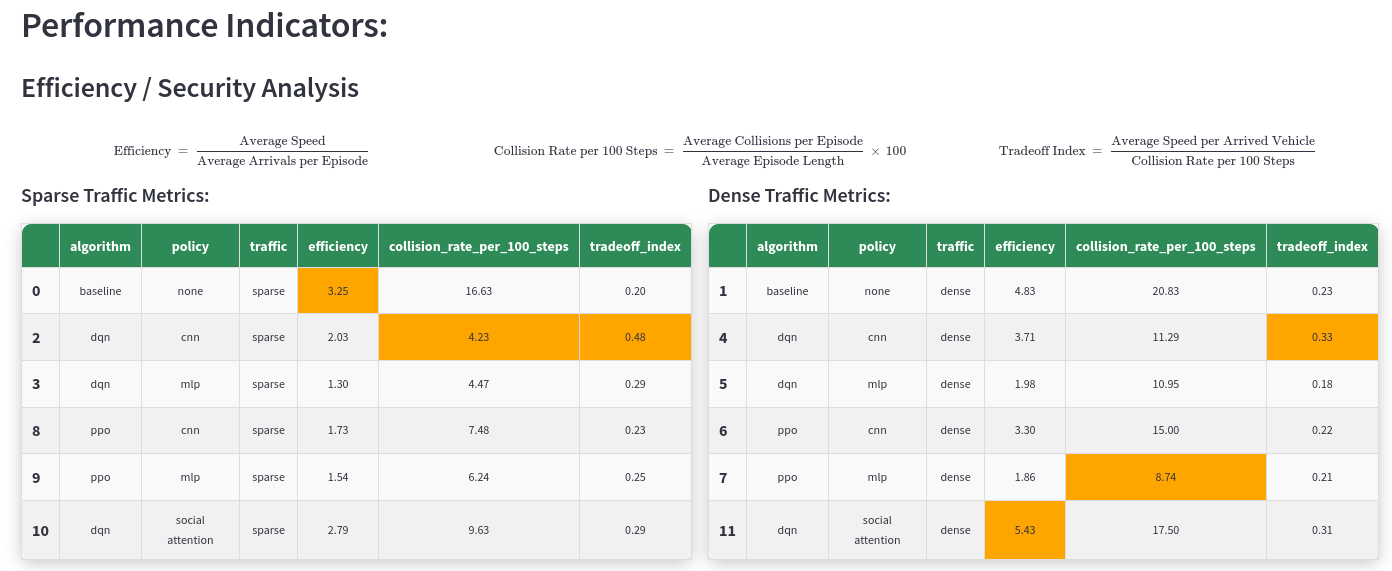
\includegraphics[height=0.3\textheight]{images/app_indicators_efficiency.png} 
    \caption{Efficiency / Security Indicators}
\end{figure}

\textbf{Efficiency/Safety Analysis}

\begin{itemize}
    \item \textbf{Efficiency} is calculated as the ratio of average speed to the average number of arrivals per episode, or inversely, the average arrivals per episode to speed. Higher efficiency values indicate better performance in terms of vehicle throughput.
    \item \textbf{Collision Rate per 100 Steps} is the rate of collisions per 100 steps in the simulation, indicating the safety of the system. A lower rate signifies better safety performance.
    \item \textbf{Tradeoff Index} represents the balance between speed and safety, with a lower value indicating better tradeoff performance (i.e., higher speed with fewer collisions).
\end{itemize}

\textbf{Sparse Traffic Metrics}

In sparse traffic, the baseline algorithm performs the best in terms of efficiency (3.25) but has a relatively high collision rate (16.63). The DQN with CNN policy shows a good balance with an efficiency of 2.03 and a lower collision rate of 4.23, making it a strong performer in sparse traffic. On the other hand, PPO algorithms, particularly with MLP, show lower efficiency and a moderate collision rate.

\textbf{Dense Traffic Metrics}

When traffic density increases, the baseline algorithm maintains its high efficiency (4.83) but faces a significant rise in the collision rate (20.83), reflecting the challenge of maintaining safety in denser traffic. The DQN with social attention policy performs notably well with high efficiency (5.43) and a lower collision rate (17.50) compared to others. In contrast, PPO algorithms continue to show lower efficiency and moderate collision rates, with PPO with MLP showing the lowest tradeoff index.

\begin{itemize}
    \item DQN with social attention seems to strike a good balance between efficiency and safety across both sparse and dense traffic scenarios.
    \item PPO algorithms, particularly with MLP, seem to struggle with efficiency and collision rate tradeoff, particularly in denser traffic.
\end{itemize}


\begin{figure}[H]
    \centering
    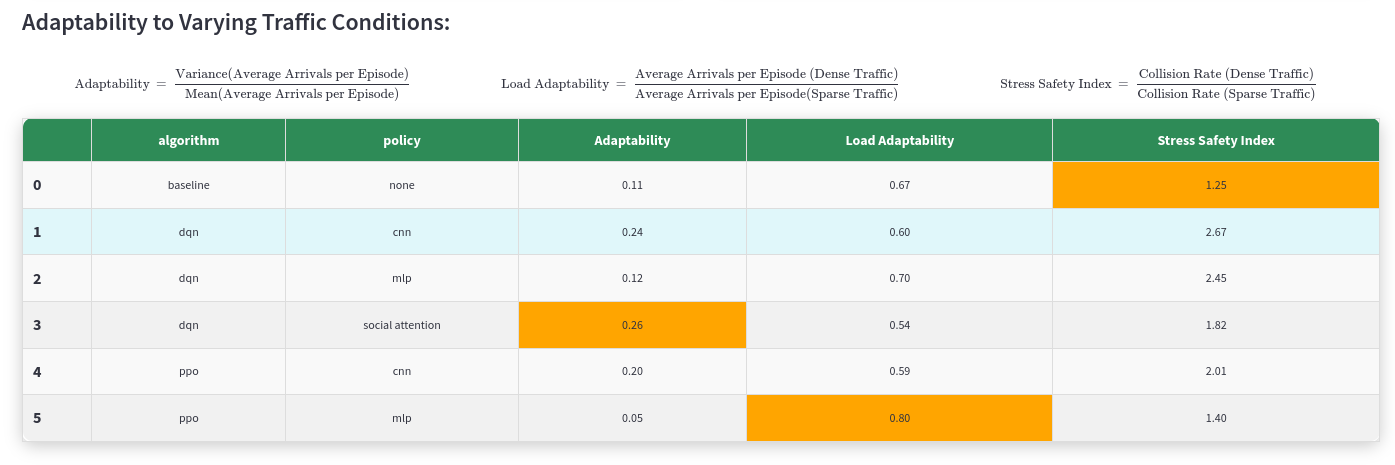
\includegraphics[height=0.25\textheight]{images/app_indicators_adapt.png} 
    \caption{Adaptability Indicators}
\end{figure}

\textbf{Adaptability to Varying Traffic Conditions}

In this analysis, three key metrics are used to assess the adaptability of different algorithms under varying traffic conditions: \textbf{Adaptability}, \textbf{Load Adaptability}, and \textbf{Stress Safety Index}.

\begin{itemize}
    \item \textbf{Adaptability}: This metric measures the variance in the number of arrivals per episode relative to the mean number of arrivals per episode. Higher values indicate better adaptability to changes in traffic conditions. Among the algorithms, the DQN with Social attention policy shows the highest adaptability with a value of 0.26, indicating better ability to adjust to fluctuating traffic conditions. The PPO with MLP policy, on the other hand, shows the lowest adaptability with a value of 0.05.
    
    \item \textbf{Load Adaptability}: This metric compares the algorithm’s performance in dense traffic to sparse traffic. 
    A higher value indicates that the algorithm performs better in dense traffic. The PPO with MLP policy exhibits the highest load adaptability (0.80), showing its ability to handle denser traffic conditions more effectively.
    In contrast, DQN with  Social attention has the lowest load adaptability (0.54), indicating lower performance in dense traffic.

    \item \textbf{Stress Safety Index}: This metric compares collision rates in dense traffic to sparse traffic. 
    A lower value indicates a better safety performance in denser traffic. The PPO with MLP policy shows the best stress safety index (1.40), indicating that it maintains lower collision rates in denser traffic compared to other algorithms. 
    DQN with CNN shows the worst performance in terms of safety, with a stress safety index of 2.67.
\end{itemize}

In summary:

\begin{itemize}
    \item DQN with Social Attention performs well in terms of adaptability, but struggles with load adaptability and stress safety.
    \item PPO with MLP is the best in terms of load adaptability and stress safety, but it has the lowest adaptability.
    \item DQN with CNN shows a balanced performance in all three metrics but does not excel in either adaptability or safety under varying traffic conditions.
\end{itemize}

This allows us to classify the algorithms into High, Medium, and Low categories based on the decision criteria.

\begin{figure}[H]
    \centering
    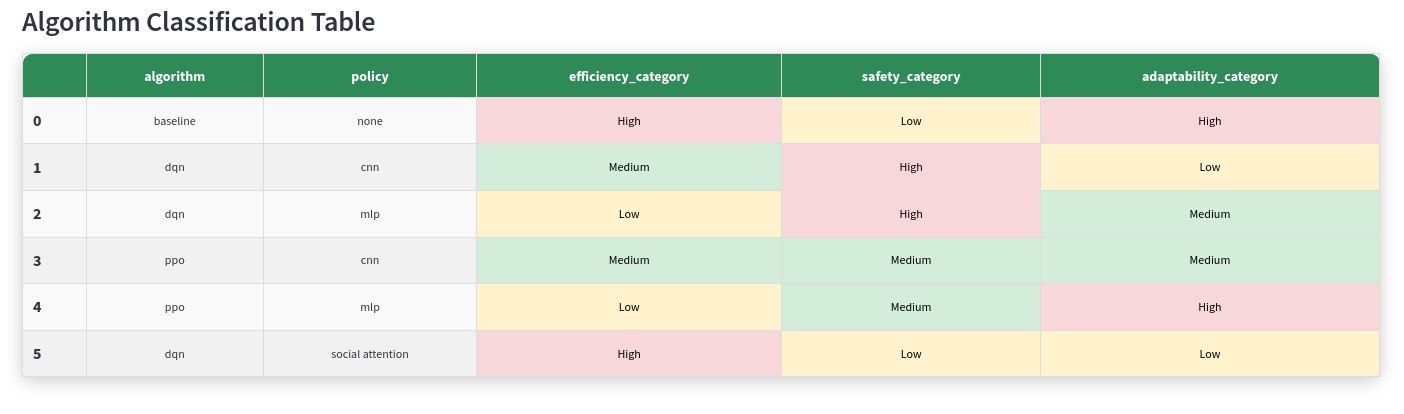
\includegraphics[height=0.22\textheight]{images/app_indicators_classif.png} 
    \caption{Algorithms Classification}
\end{figure}

\textbf{Efficiency:}  
The DQN algorithm with the social attention policy is categorized as \textit{High} in efficiency, indicating its exceptional performance.  
The DQN with CNN and PPO with CNN are classified as \textit{Medium} in efficiency, while the DQN with MLP and PPO with MLP are placed in the \textit{Low} category, reflecting their subpar efficiency.

\textbf{Safety:}  
The DQN with CNN policy excels in safety, earning a \textit{High} classification.  
On the other hand, the DQN with Social Attention and PPO with MLP fall into the \textit{Low} safety category.  
PPO with CNN and DQN with MLP are categorized as \textit{Medium}, indicating an average level of safety.

\textbf{Adaptability:}  
Both the Baseline and PPO with MLP algorithms are classified as \textit{High} in adaptability, showcasing strong performance across varying traffic conditions.  
The DQN with CNN, PPO with CNN, and DQN with MLP are rated as \textit{Medium} in adaptability, while the DQN with Social Attention is ranked \textit{Low} in this metric.

To summarize, The \textbf{DQN} with CNN offers a balanced performance, achieving medium efficiency, high safety, but low adaptability. 
Conversely, the \textbf{PPO} algorithms underperform in both efficiency and adaptability, though they maintain average safety levels. 
Finally, the \textbf{DQN} with Social attention demonstrates good efficiency but is limited by poor adaptability and safety performance.


\chapter{Conclusions and Future Work}
\section{Conclusions}

This project has successfully developed and evaluated a robust and adaptable Multi-Agent System (MAS) for managing autonomous vehicles at road intersections. The primary objectives of the project were to train agents using Deep Reinforcement Learning (DRL) algorithms, evaluate their performance under various traffic conditions, and assess the scalability and robustness of the system.

In the first phase, the agents were trained using a set of DRL algorithms, such as DQN and PPO, to enable autonomous decision-making regarding intersection crossing orders and speed control. The goal was to optimize traffic flow while ensuring that the agents avoid collisions. The training phase was successful, with agents demonstrating the ability to navigate the intersection effectively, adjust their speeds, and follow traffic rules.

In the second phase, the impact of different traffic flow configurations (sparse and dense traffic) on the agents' performance was explored. The evaluation revealed that some algorithms, particularly DQN with Social Attention, demonstrated superior adaptability to the varying traffic densities. In dense traffic scenarios, some algorithms exhibited challenges in maintaining safety and efficiency, leading to higher collision rates and shorter episode lengths.

The third phase of the project focused on evaluating the system's scalability and robustness. The metrics collected during this phase provided valuable insights into how different algorithms perform across multiple simulations with varying environmental conditions. The results showed that while some algorithms like DQN with Social Attention excelled in both efficiency and safety, others, such as PPO, struggled with adaptability under varying traffic conditions.

Overall, the project successfully achieved its objectives by training autonomous agents, evaluating their performance in different environments, and analyzing the scalability and robustness of the system. The classification of algorithms into performance categories such as efficiency, safety, and adaptability provides a clear understanding of each algorithm's strengths and weaknesses.

\section{Future Work}

While this project has provided valuable insights into the performance of different DRL algorithms for managing autonomous vehicles at intersections, there are several areas where future work could further enhance the system:

\begin{itemize}
    \item \textbf{Exploring Additional DRL Algorithms}: Future work can investigate the use of more advanced DRL algorithms, such as A3C (Asynchronous Advantage Actor-Critic) or TRPO (Trust Region Policy Optimization), to further improve the learning efficiency and performance of the agents. These algorithms might offer better stability or faster convergence compared to the ones used in this study.
    \item \textbf{Handling Complex Traffic Scenarios}: Future experiments could involve simulating more complex traffic environments, such as intersections with multiple lanes, traffic lights, or various types of vehicles. Introducing more variables could provide a more comprehensive test of the system's robustness and adaptability.
    \item \textbf{Real-Time Agent Adaptation}: Enhancing the agents' ability to adapt in real-time to sudden changes in traffic patterns (e.g., unexpected vehicle arrivals, accidents, or emergency vehicle scenarios) could be explored. Implementing techniques such as online learning or meta-learning could allow the agents to update their policies during execution.
    \item \textbf{Integration with Real-World Simulations}: Future research could focus on transferring the learned models to real-world environments, using simulations that closely resemble actual traffic intersections. This would involve integrating sensor data, real-time decision-making, and safety protocols for real-world deployment.
    \item \textbf{Performance Evaluation in Mixed Traffic Conditions}: Exploring how the trained agents perform in mixed traffic environments with both human-driven and autonomous vehicles would be essential for real-world applications. This could include the analysis of how well the agents cooperate with human drivers or adapt to their actions.
\end{itemize}

By addressing these areas, the system can be further refined, improving its capabilities in real-world applications for managing autonomous vehicles and contributing to the broader field of intelligent transportation systems.

% References
\printbibliography

% Appendices
\appendix
\chapter{Appendix: Deploying the App}
\subsection*{Running the train and test code}

In order to run the Python train and test code follow these steps:

\textbf{Set up the environment:} Ensure that Python is installed, and create a virtual environment to manage dependencies.
(\texttt{virtualenv}, \texttt{pyenv} or \texttt{conda} can be used for this).

\begin{verbatim}
    $ cd Train_and_Test_code
    $ pip install -r requirements.txt
\end{verbatim}


\begin{verbatim}
    $ python train_intersection_dqn_cnn_multi.py
\end{verbatim}

The train generated models will be stored in a subdirectory \textbf{models}

\textbf{Required Python Packages:} (Listed on \textit{requirements.txt}):
\begin{quote}

    gymnasium==1.0.0

    highway\-env==1.10.1

    rl-agents==1.0.dev0

    stable\_baselines3==2.3.2

\end{quote}




\end{document}


